\documentclass[11pt,a4paper]{article}
\usepackage{listings}
\usepackage[utf8]{inputenc}
\usepackage{mathtools}
\usepackage[norsk]{babel}
\usepackage{graphicx}
\usepackage{gensymb}
\usepackage{wasysym}
\usepackage{hyperref}
\usepackage{setspace}
\usepackage{tikz}
\usepackage{amsthm}
\usepackage{amsmath}
\usepackage{mathrsfs}
\usepackage{amssymb}
\usepackage{color}
\usepackage{rotating}
\usepackage{pgfplots}
\usepackage{algorithmicx}
\usepackage{fancyvrb}

\usepackage[margin=2.5cm]{geometry}

% Two column table of content
\usepackage[toc]{multitoc}
\renewcommand*{\multicolumntoc}{2}
\setlength{\columnseprule}{0.5pt}


\usetikzlibrary{arrows}
\usetikzlibrary{shapes, automata}
 
\definecolor{dkgreen}{rgb}{0,0.6,0}
\definecolor{gray}{rgb}{0.5,0.5,0.5}
\definecolor{mauve}{rgb}{0.58,0,0.82}


\lstset{ %
  language=Java,                % the language of the code
  basicstyle=\small\ttfamily,           % the size of the fonts that are used for the code
  numbers=none,                   % where to put the line-numbers
  numberstyle=\small\color{gray},  % the style that is used for the line-numbers
  stepnumber=1,                   % the step between two line-numbers. If it's 1, each line 
                                  % will be numbered
  numbersep=5pt,                  % how far the line-numbers are from the code
  backgroundcolor=\color{white},      % choose the background color. You must add \usepackage{color}
  showspaces=false,               % show spaces adding particular underscores
  showstringspaces=true,         % underline spaces within strings
  showtabs=false,                 % show tabs within strings adding particular underscores
  frame=false,                   % adds a frame around the code
  rulecolor=\color{white},        % if not set, the frame-color may be changed on line-breaks within not-black text (e.g. commens (green here))
  tabsize=2,                      % sets default tabsize to 2 spaces
  captionpos=b,                   % sets the caption-position to bottom
  breaklines=true,                % sets automatic line breaking
  breakatwhitespace=false,        % sets if automatic breaks should only happen at whitespace
  title=\lstname,                   % show the filename of files included with \lstinputlisting;
                                  % also try caption instead of title
  keywordstyle=\bfseries\color{blue},          % keyword style
  commentstyle=\color{dkgreen},       % comment style
  stringstyle=\color{mauve},         % string literal style
  escapeinside={\%*}{*)},            % if you want to add LaTeX within your code
  morekeywords={*,..,function}               % if you want to add more keywords to the set
}

\setlength{\parskip}{5mm}

\newtheoremstyle{def}
	{3pt}	% Space above
	{3pt}	% Space below
	{\itshape}		% Font
	{}		% Indent
	{\bfseries}		% Head font
	{:}		% Head punct.
	{.5em}	% Space after head
	{}		% Head spec

\theoremstyle{def}
\newtheorem{definition}[subsection]{Definisjon}

%\newenvironment{definition}[1][Definisjon]{\begin{trivlist}
%\item[\hskip \labelsep {\bfseries #1}]}{\end{trivlist}}

\title{Notater: INF2220}
\author{Veronika Heimsbakk \\ 
veronahe@ifi.uio.no}
\begin{document}

\maketitle{}
\tableofcontents

\section*{Introduksjon}
Dette er notater til kurset INF2220--Algoritmer og datastrukturer\cite{inf2220} ved Universitetet i Oslo. Disse notatene er i all hovedsak basert på forelesningsfoiler, egne notater og læreboka. Brukes til repetisjon før eksamen og som notater under eksamen. Merk at notatene helt sikkert inneholder feil og mangler.

\newpage

%%% KJØRETID %%%
\section{Kjøretid}

\begin{definition}
\emph{\textbf{O-notasjon}}
La $f$ og $g$ være funksjoner $f,g: \mathcal{N} \rightarrow \mathcal{R}^+$. Sier at $\textbf{f(n) = O(g(n))}$ hvis det eksisterer positive heltall $c$ og $n_0$ slik at for hvert heltall $n \geq n_0$,
$$f(n) \leq c g(n).$$
Når $f(n) = O(g(n))$, sier vi at $g(n)$ er \textbf{upper bound} for $f(n)$, eller mer presist at $g(n)$ er \textbf{asymptotic upper bound} for $f(n)$.
\end{definition}

\begin{minipage}{0.35\textwidth}
\begin{tabular}{rl}
\textbf{Funksjon}&\textbf{Navn}\\
$1$&Konstant\\
$\log n$&Logaritmisk\\
$n$&Lineær\\
$n \log n$&\\
$n^2$&Kvadratisk\\
$n^3$&Kubisk\\
$2^n$&Eksponensiell\\
$n!$&\\
\end{tabular}
\end{minipage}
\begin{minipage}{0.5\textwidth}
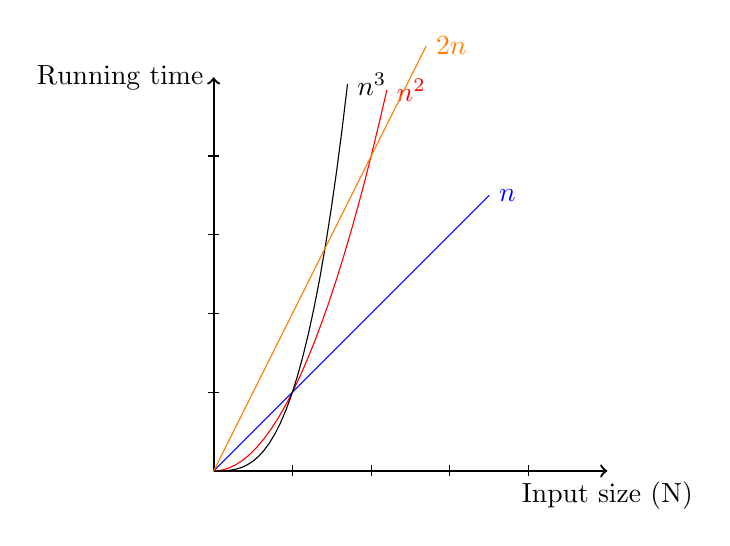
\begin{tikzpicture}
\draw[thick, ->] (0,0) -- (5,0) node[below] {Input size  (N)};
\draw[thick, ->] (0,0) -- (0,5) node[left] {Running time};

\foreach \x in {1,2,3,4}
	\draw (\x cm, 2pt) -- (\x cm, -2pt);
\foreach \y in {1,2,3,4}
	\draw (2pt, \y cm) -- (-2pt, \y cm);

\draw[red, domain=0:2.2] plot (\x, {\x^2}) node[right]{$n^2$};
\draw[blue, domain=0:3.5] plot (\x, {\x}) node[right] {$n$};
\draw[black, domain=0:1.7] plot (\x, {\x^3}) node[right] {$n^3$};
\draw[orange, domain=0:2.7] plot (\x, {2*\x}) node [right] {$2n$};
\end{tikzpicture}
\end{minipage}

\subsection{Analyse av kjøretid}
Når man analyserer en algoritme, så må man se på \textit{stegene} den bruker og analysere de hver for seg. Ta for eksempel denne kodesnutten:
\begin{lstlisting}
for (i = 0; i < n; i++)
  for (j = 0; j < m; j++)
    array[i][j] = 0;
\end{lstlisting}
\vspace{-20pt}

\noindent To steg:\vspace{-15pt}
\begin{enumerate}
\item
Ytterste løkke går i O(n).
\item
Innerte løkke går i O(m).
\end{enumerate}
\vspace{-15pt}
Dette gir O(n) $\times$ O(m) = O(n$^2$).

\subsection{Logaritmisk tid}
Algoritmer som tar logaritmisk tid, O$(\log n)$, finner man i operasjoner på binære trær, eller når man bruker binære søk og i \textit{divide and conquer}-algoritmer. 

\begin{lstlisting}
for (i = 1; i < n; i = i * 2)
    sum++;
\end{lstlisting}
\vspace{-15pt}

\newpage

%%% TRÆR %%%
\section{Trær}

\begin{definition}
\emph{\textbf{Tre}}
Et \textbf{tre} er en samling \textbf{noder}. Et ikke-tomt tre består av en \textbf{rot}-node, og null eller flere ikke-tomme \textbf{subtrær}. Fra roten går en \textbf{rettet kant} til roten i hvert subtre.
\end{definition}

% Traversering
\subsection{Traversering}
\begin{description}
\item[Pre-order] rot, venstre barn, høyre barn
\item[In-order] venstre barn, rot, høyre barn
\item[Post-order] venstre barn, høyre barn, rot
\end{description}

\begin{lstlisting}[frame=none]
/* IN-ORDER TRAVERSAL */

public void inOrder (Node node) {
	if (node != null) {
		inOrder(node.left);
		// do something with the node
		inOrder(node.right);
	}
}

/* PRE-ORDER TRAVERSAL */

public void preOrder (Node node) {
	if (node != null) {
		// do something with the node
		preOrder(node.left);
		preOrder(node.right);
	}
}

/* POST-ORDER TRAVERSAL */

public void postOrder (Node node) {
	if (node != null) {
		postOrder(node.left);
		postOrder(node.right);
		// do something with the node
	}
}
\end{lstlisting}

\vspace{-25pt}

% Terminologi
\subsection{Terminologi}
\begin{definition}
\emph{\textbf{Sti}}
En sti fra node $n_1$ til $n_k$ er definert som en sekvens $n_1, n_2, \dots, n_k$, slik at $n_i$ er forelder til $n_{i+1}$ for $1 \leq i \leq k$.
\end{definition}
\begin{definition}
\emph{\textbf{Lengde}}
Antall \textit{kanter} på veien; $k-1$.
\end{definition}
\begin{definition}
\emph{\textbf{Dybde}}
Definert av den unike veien fra roten til noden. Rotens dybde er 0.
\end{definition}
\begin{definition}
\emph{\textbf{Høyde}}
Definert som lengden av den \textit{lengste} veien fra noden til en løvnode. Alle løvnoder har høyde 0. Høyden til et tre er lik høyden til roten.
\end{definition}

%%% BINÆRTRÆR %%%
\subsection{Binært søketre}

\begin{definition}
\emph{\textbf{Binært søketre}}
Et binært søketre (BST) er et \textbf{ordnet} binært tre. Følgende kriterier må være oppfylt for at treet skal være et BST:
\begin{itemize}
\item
Verdiene i \textbf{venstre} subtre er \textbf{mindre} enn noden i seg selv.
\item
Verdiene i \textbf{høyre} subtre er \textbf{større} enn noden i seg selv.
\item
Venstre og høyre subtre må også være binære søketrær.
\item
Hver node kan ha maksimum to barn.
\item
Det eksisterer en \textbf{unik} sti fra roten til enhver node i treet.
\end{itemize}
\end{definition}

\begin{figure}[h!]
\centering
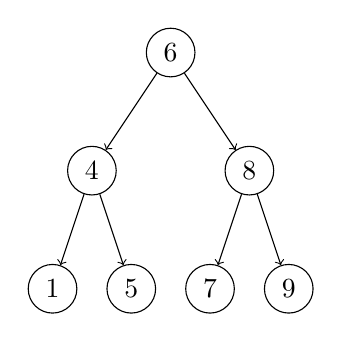
\begin{tikzpicture}[->,every node/.style={circle, draw=black}, 
				   level 1/.style={sibling distance=20mm},
				   level 2/.style={sibling distance=10mm}]
\node{6}
	child {node {4}
		child {node {1}}
		child {node {5}}
	}
	child {node {8}
		child {node {7}}
		child {node {9}}
	}
;
\end{tikzpicture}
\label{fig:simplebst}
\caption{Eksempel på et binært søketre.}
\end{figure}

\begin{table}[h!]
\centering
\begin{tabular}{rll}
&Average&Worst case\\
\textbf{Plass} & O($n$) & O($n$)\\
\textbf{Søk} & O($\log n$) & O($n$)\\
\textbf{Innsetting} & O($\log n$) & O($n$)\\
\textbf{Sletting} & O($\log n$) & O($n$)\\
\end{tabular}
\label{tab:obst}
\caption{Tidkompleksitet for BST.}
\end{table}

\subsubsection{Søking}
\begin{lstlisting}
function find(key, node):
  if node = Null or node.key = key then
    return node
  else if key < node.key then
    return find(key, node.left)
  else
    return find(key, node.right)
\end{lstlisting}

\vspace{-25pt}

\subsubsection{Sette inn}
\begin{lstlisting}
function insert(root, data):
  if (!root)
    root = new Node(data)
  else if (data < root.data)
    insert(root.left, data)
  else if (data > root.data)
    insert(root.right, data)
\end{lstlisting}

\subsubsection{Fjerne element}

\begin{itemize}
\item
\textbf{Noden er en løvnode}: kan fjernes direkte.
\item
\textbf{Noden har bare ett barn}: foreldrenoden kan enkelt hoppe over den som skal fjernes.
\item
\textbf{Noden har to barn}: erstatt verdien i noden med den misnte verdien i høyre subtre. Slett noden som denne minste verdien var i.
\end{itemize}

\begin{lstlisting}[frame=none]
public boolean remove (int key) {
	Node current, parent = root;
	boolean isALeft = true;

	while (current.key != key) {
		parent = current;

		if (key < current.key) {
			isALeft = true;
			current= current.left;
		}
		else {
			isALeft = false;
			current = current.right;
		}
		if (current == null)
			return false;
	}

	if (current.left == null && current.right == null) {
		if (current == root)
			root == null;
		else if (isALeft)
			parent.left = null;
		else 
			parent.right = null;
	}
	else if (current.left == null) {
		if (current == root)
			root = current.right;
		else if (isALeft)
			parent.left = current.right;
		else
			parent.right = current.left;
	}
	else {
		Node replacement = replace(current);
	
		if (current == root)
			root = replacement;
		else if (isALeft)
			parent.left = replacement;
		else
			parent.right = replacement;
		replacement.left = current.left;
	}
	return true;
}

public Node replace (Node replaceNode) {
	Node replaceParent = replaceNode;
	Node replacement = replaceNode;
	Node current = replaceNode.right;

	while (current != null) {
		replaceParent = replacement;
		replacement = current;
		current = current.left;
	}
	if (replacement != replaceNode.right) {
		replaceParent.left = replaceNode.right;
		replaceNode.right = replacement.right;
	}
	return replaceNode;
}
\end{lstlisting}
\vspace{-30pt}


%%% Rød-svarte trær
\subsection{Rød-svarte trær}
\begin{definition}
\emph{\textbf{Rød-svart tre}}
En datastruktur som er et \textbf{selv-balanserende} binært søketre. Følgende skal gjelde for et rød-svart tre:
\begin{enumerate}
\vspace{-15pt}
\item
En node er enten rød eller sort.
\item
Roten er sort.
\item
Alle løvnoder (NIL) er sorte---alle løvnoder har samme farge som roten.
\item
Enhver røde node må ha to sorte barn.
\item
Enhver sti fra roten til en løvnode skal inneholde samme antall sorte noder.
\vspace{-15pt}
\end{enumerate}
Dette sikrer at høyden på et slikt tre er maks $2\times\log_2(N+1)$.
\end{definition}


\tikzset{
	treenode/.style = {align=center, inner sep=-8pt},
	% Sorte noder
	node_black/.style = {treenode, circle, white,
						font=\bfseries, draw=black,
						fill=black, text width=0.5cm},
	% Røde noder
	node_red/.style = {treenode, circle, red, fill=red,
						text width=0.5cm, very thick},
	% Null-pekere
	node_null/.style = {white, treenode, rectangle, draw=black, fill=black,
						minimum width=0.3cm, minimum height=0.3cm}
}

\subsubsection{Situasjoner som kan oppstå.}
Det er tre situasjoner som kan oppstå i rød-svarte trær.

\begin{enumerate}
\vspace{-15pt}
\item
Onkelen er rød, skal da bytte farge mellom besteforelder og forelder/onkel.
\item
Høyre og venstre eller venstre og høyre, rotér forelder, så rotér besteforelder.
\item
Høyre og høyre eller venste og venstre, så rotér besteforelder.
\end{enumerate}


\begin{minipage}{0.35\textwidth}
\begin{tabular}{lll}
&\textbf{Case 1}&$\rightarrow$\\
&
\begin{tikzpicture}[scale=0.6]
\node[node_black] {}
	child {node[node_red] {}
		child {node[node_red] {}}
		child[white] {node[fill=white] {}}
	}
	child {node[node_red] {}}
;
\end{tikzpicture}
&
\begin{tikzpicture}[scale=0.6]
\node[node_red] {}
	child {node[node_black] {}
		child {node[node_red] {}}
		child[white] {node[fill=white] {}}
	}
	child {node[node_black] {}}
;
\end{tikzpicture}\\
\end{tabular}
\end{minipage}
\begin{minipage}{0.5\textwidth}
Bytter farger, men må farge roten tilbake til svart igjen.
\end{minipage}

\begin{minipage}{0.6\textwidth}
\begin{tabular}{lllll}
&\textbf{Case 2}&eller&&$\rightarrow$\\
&
\begin{tikzpicture}[scale=0.6]
\node[node_black] {}
	child {node[node_red] {}
		child[white] {node[fill=white] {}}
		child {node[node_red] {}}
	}
	child {node[node_black] {}}
;
\end{tikzpicture}
&
\begin{tikzpicture}[scale=0.6]
\node[node_red] {}
	child {node[node_black] {}}
	child {node[node_black] {}
		child {node[node_red] {}}
		child[white] {node[fill=white] {}}
}
;
\end{tikzpicture}
&
\begin{tikzpicture}[scale=0.6]
\node[node_black] {}
	child {node[node_red] {}
		child[white] {node[fill=white] {}}
		child {node[node_red] {}}
	}
	child {node[node_black] {}}
;
\end{tikzpicture}
&
\begin{tikzpicture}[scale=0.6]
\node[node_red] {}
	child {node[node_red] {}}
	child {node[node_black] {}
		child[white] {node[fill=white] {}}
		child {node[node_black] {}}
}
;
\end{tikzpicture}\\
\end{tabular}
\end{minipage}
\begin{minipage}{0.4\textwidth}
Roterer forelder, så besteforelder. Må fargelegge om etter rotering.
\end{minipage}

\begin{minipage}{0.35\textwidth}
\begin{tabular}{lll}
&\textbf{Case 3}&$\rightarrow$\\
&
\begin{tikzpicture}[scale=0.6]
\node[node_black] {}
	child {node[node_red] {}
		child {node[node_red] {}}
		child[white] {node[fill=white] {}}
	}
	child {node[node_black] {}}
;
\end{tikzpicture}
&
\begin{tikzpicture}[scale=0.6]
\node[node_red] {}
	child {node[node_red] {}}
	child {node[node_black] {}
		child[white] {node[fill=white] {}}
		child {node[node_black] {}}
}
;
\end{tikzpicture}\\
\end{tabular}
\end{minipage}
\begin{minipage}{0.5\textwidth}
Rotasjon på besteforelder. Må fargelegge om etter rotasjonen.
\end{minipage}
 
\begin{figure}[h!]
\begin{lstlisting}[frame=single]
/* Red-black insertion */

public void put (Key key, Value val) {
	root = put(root, key, val);
	root.color = BLACK;
}

// insert key-value pair in subtree with root node
private Node put (Node node, Key key, Value val) {
	if (node == null) return new Node(key, val, RED, 1);

	int cmp = key.compareTo(node.key);
	if (cmp < 0) 
		node.left = put(node.left, key, val);
	if else (cmp > 0)
		node.right = put (node.right), key, val);
	else 
		node.val = val;

	if ( isRed(node.right) && !isRed(node.left) ) 
		node = rotateLeft(node);
	if ( isRed(node.left) && isRed(node.left.left) ) 
		node = rotateRight(node);
	if ( isRed(node.left) && isRed(node.right) ) 
		flipColors(node);
	node.N = size(node.left) + size(node.right) + 1;

	return node;
}
\end{lstlisting}
\vspace{-15pt}
\caption{Eksempel på innsetting i rødsvart tre \cite{redblack}.}
\end{figure}

\begin{table}[h!]
\centering
\begin{tabular}{rll}
&Average&Worst case\\
\textbf{Plass} & O($n$) & O($n$)\\
\textbf{Søk} & O($\log n$) & O($\log n$)\\
\textbf{Innsetting} & O($\log n$) & O($\log n$)\\
\textbf{Sletting} & O($\log n$) & O($\log n$)\\
\end{tabular}
\label{tab:obst}
\caption{Tidkompleksitet for rød-svarte trær.}
\end{table}

\newpage

%%% B-TRÆR %%%
\subsection{B-trær}
\vspace{-10pt}
Kravene til et B-tre er følgende:
\begin{itemize}
\vspace{-20pt}
\item
Alle data er lagret i løvnodene.
\item
Roten har mellom \textbf{2} og \textbf{M} barn. 
\item
Alle løvnoder har mellom \textbf{L/2} og \textbf{L} elementer.
\end{itemize}


\paragraph{Eksempel på innsetting i B-tre} Sette inn tallene 2, 6, 17, 20, 24, 25, 27, 29, 30, 31, 32, 5, 21, 1, 40, 45, 50, 70 med kravene M = 5, L = 5.

\begin{minipage}{0.5\textwidth}
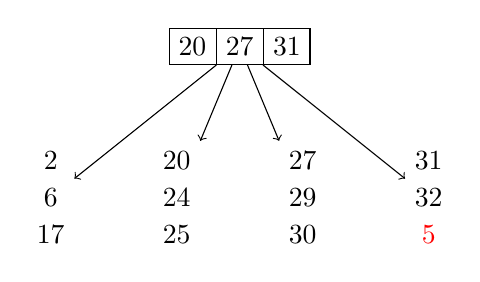
\begin{tikzpicture}[scale=0.8, every node/.style = {rectangle split ignore empty parts},
					level 1/.style = {sibling distance=20mm},
					level 2/.style = {sibling distance=15mm}]

\tikzstyle{leaf}=[rectangle split, below]
\tikzstyle{normal_node} = [rectangle split, rectangle split horizontal,draw]

\node[normal_node] {20 \nodepart{two} 27 \nodepart{three} 31} [->]
	child {node[leaf] {2 \nodepart{two} 6 \nodepart{three} 17}}
	child {node[leaf] {20 \nodepart{two} 24 \nodepart{three} 25}}
	child {node[leaf] {27 \nodepart{two} 29 \nodepart{three} 30}}
	child {node[leaf] {31 \nodepart{two} 32 \nodepart{three} \textcolor{red}{5}}}
;
\end{tikzpicture}
\end{minipage}
\begin{minipage}{0.5\textwidth}
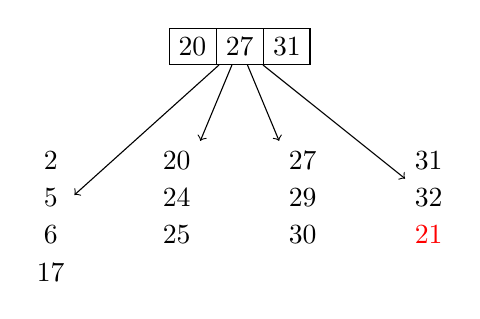
\begin{tikzpicture}[scale=0.8,every node/.style = {rectangle split ignore empty parts},
					level 1/.style = {sibling distance=20mm},
					level 2/.style = {sibling distance=15mm}]

\tikzstyle{leaf}=[rectangle split, below]
\tikzstyle{normal_node} = [rectangle split, rectangle split horizontal,draw]

\node[normal_node] {20 \nodepart{two} 27 \nodepart{three} 31} [->]
	child {node[leaf] {2 \nodepart{two} 5 \nodepart{three} 6 \nodepart{four} 17}}
	child {node[leaf] {20 \nodepart{two} 24 \nodepart{three} 25}}
	child {node[leaf] {27 \nodepart{two} 29 \nodepart{three} 30}}
	child {node[leaf] {31 \nodepart{two} 32 \nodepart{three} \textcolor{red}{21}}}
;
\end{tikzpicture}
\end{minipage}
\begin{minipage}{0.5\textwidth}
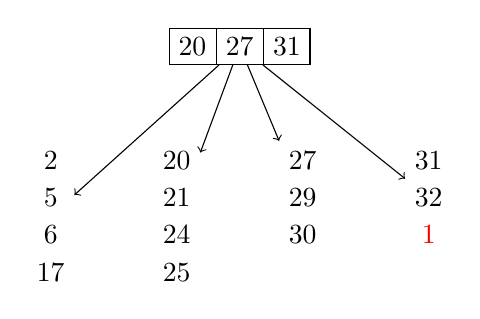
\begin{tikzpicture}[scale=0.8,every node/.style = {rectangle split ignore empty parts},
					level 1/.style = {sibling distance=20mm},
					level 2/.style = {sibling distance=15mm}]

\tikzstyle{leaf}=[rectangle split, below]
\tikzstyle{normal_node} = [rectangle split, rectangle split horizontal,draw]

\node[normal_node] {20 \nodepart{two} 27 \nodepart{three} 31} [->]
	child {node[leaf] {2 \nodepart{two} 5 \nodepart{three} 6 \nodepart{four} 17}}
	child {node[leaf] {20 \nodepart{two} 21 \nodepart{three} 24 \nodepart{four} 25}}
	child {node[leaf] {27 \nodepart{two} 29 \nodepart{three} 30}}
	child {node[leaf] {31 \nodepart{two} 32 \nodepart{three} \textcolor{red}{1}}}
;
\end{tikzpicture}
\end{minipage}
\begin{minipage}{0.5\textwidth}
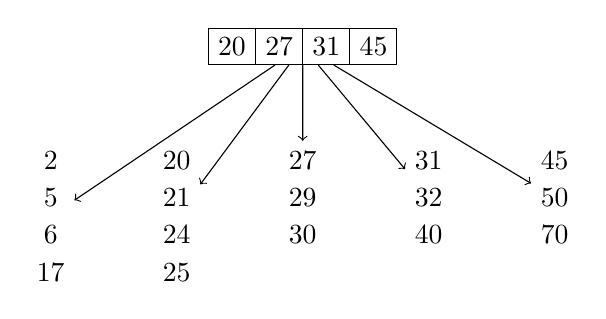
\begin{tikzpicture}[scale=0.8,every node/.style = {rectangle split ignore empty parts},
					level 1/.style = {sibling distance=20mm},
					level 2/.style = {sibling distance=15mm}]

\tikzstyle{leaf}=[rectangle split, below]
\tikzstyle{normal_node} = [rectangle split, rectangle split horizontal,draw]

\node[normal_node] {20 \nodepart{two} 27 \nodepart{three} 31 \nodepart{four} 45} [->]
	child {node[leaf] {2 \nodepart{two} 5 \nodepart{three} 6 \nodepart{four} 17}}
	child {node[leaf] {20 \nodepart{two} 21 \nodepart{three} 24 \nodepart{four} 25}}
	child {node[leaf] {27 \nodepart{two} 29 \nodepart{three} 30}}
	child {node[leaf] {31 \nodepart{two} 32 \nodepart{three} 40}}
	child {node[leaf] {45 \nodepart{two} 50 \nodepart{three} 70}}
;
\end{tikzpicture}
\end{minipage}

Når den ene løvnoden fylles opp til maks antall elementer, så må den splittes i halv til to nye løvnoder.


\paragraph{Sletting fra B-tre}
\begin{enumerate}
\item
Finn riktig løvnode for tallet som skal slettes ved søking.
\item
Hvis løvnoden har minst \textbf{L/2+1} elementer, kan vi enkelt slette tallet.
\item
Hvis ikke, må løvnoden kombineres med en av nabonodene.
\begin{enumerate}
\item
Hvis venstre/høyre søsken har minst \textbf{L/2+1} elementer, flytter vi det største/minste elementet over til løvnoden.
\item
Hvis søsken har akkurat \textbf{L/2} elementer, slår vi de to nodene sammen til en node (med L eller L-1 elementer).
\end{enumerate}
\item
Gjenta punkt 3 dersom foreldrenoden har ett barn.
\item
Til slutt: hvis roten bare har ett barn, slettes denne og barnet blir ny rot.
\end{enumerate}
Husk å oppdatere nøkkelverdiene underveis!

\newpage

%%% HASHING %%%
\section{Hashing}
Idéen i hashing er å lagre alle elementene i en array (hashtabell) og la verdien i elementet $x$ bestemme indeksen til $x$ i hashtabellen. Egenskaper til en god hash-funksjon er at den er rask å beregne, kan gi alle mulige verdier fra 0 til tabellens størrelse $-1$. Og den git en god fordeling utover tabellindeksene. En hashtabell tilbyr innsetting, sletting og søking med konstant tid.

\subsection{Hash-funksjoner}
\paragraph{Eksempel} med heltall som nøkkel, begrenset antall tabellindekser. La hashfunksjonen være \texttt{hash(x, taleSize) = x mod tableSize}. Husk at hvis \texttt{tableSize} er 10 og alle nøklene slutter på 0, vil alle elementene havne på samme indeks. Huskeregel for dette: la alltid tabellstørrelsen være et primtall. Funksjonen under summerer verdiene til hver bokstav. Dette er en dårlig fordeling dersom tabellstørrelsen er stor.
\begin{lstlisting}
int hash (String key, int tableSize) {
	int hashValue = 0;
	for (i = 0; i < key.length(); i++) 
		hashValue+= key.charAt(i);
	return (hashValue % tableSize);
}
\end{lstlisting}
\vspace{-45pt}

\subsection{Forskjellige typer hash-tabeller}
\begin{itemize}
\item
\textbf{Seprate chaining} er en hash-tabell hvor hver indeks peker til en liste av elementer.
\item
\textbf{Probing} er rommet mellom hver indeks.
\begin{itemize}
\item
\textit{Lineær probing}: intervallene er satt (normalt 1).
\item
\textit{Kvadratisk probing}: intervallene øker med å legge til et kvadratisk polynom ($1^2=1, 2^2=4, 3^2=5,\dots$ ved startverdi gitt av hashberegningen.
\item
\textit{Dobbel hashing}: intervallene er gitt av en annen hash-funksjon. \texttt{H$_2$(X) = R-(X mod R)}, hvor \texttt{R} er det største primtallet som er \textit{mindre} enn tabellstørrelsen.
\end{itemize}
\end{itemize}

\begin{table}[h!]
\centering
\begin{tabular}{c|c|c|c}
Index & Linear probing & Quadratic probing & Separate chaining\\
\hline
0 & 9679 & 9679 &\\
1 & 4371 & 4371 & \\
2 & 1989 & &\\
3 & 1323 & 1323 & 1323 $\rightarrow$ 6173\\
4 & 6173 & 6173 & 4344\\
5 & 4344 & 4344 &\\
6 & & &\\
7 & & &\\
8 & & 1989 &\\
9 & 4199 & 4199 & 4199 $\rightarrow$ 9679 $\rightarrow$ 1989\\
\end{tabular}
\label{tab:hash}
\caption{Eksempel på hashing.}
\end{table}
I tabell \ref{tab:hash} har vi forskjellige hash-tabeller på tallene \{4371, 1323, 4199, 4344, 9679, 1989\} som skal settes inn i en tabell på størrelse 10, og med hash-funksjon \texttt{H(X) = X mod 10}.

%%% HEAP %%%
\section{Heap}

En \textbf{binær heap} er et komplett binærtre, hvor barna alltid er større eller lik sine foreldre. Og et komplett binærtre har følgende egenskaper:

\begin{itemize}
\item
Treet vil være i perfekt balanse.
\item
Løvnoder vil ha høydeforskjell på maksimalt 1.
\item
Treet med høyden $h$ har mellom $2^h$ og $2^{h+1}-1$ noder.
\item
Den maksimale høyden på treet vil være $\log_2(n)$.
\end{itemize}

\subsection{Eksempel på sletting i min-heap}
Skal gjøre operasjonen \texttt{deleteMin()} på følgende heap.

\begin{minipage}{0.5\textwidth}
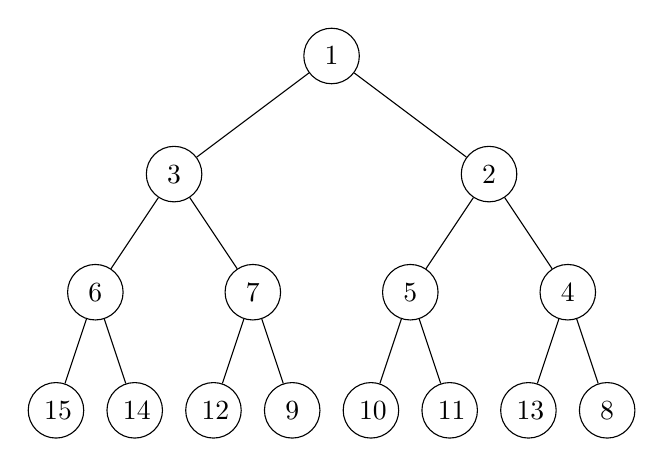
\begin{tikzpicture}[every node/.style={circle, draw=black, text width=0.3cm, align=center},
				   level 1/.style={sibling distance=40mm},
				   level 2/.style={sibling distance=20mm},
				   level 3/.style={sibling distance=10mm}]
\node{1}
	child {node {3}
		child {node {6}
			child {node {15}}
			child {node {14}}
		}
		child {node {7}
			child {node {12}}
			child {node {9}}
		}
	}
	child {node {2}
		child {node {5}
			child {node {10}}
			child {node {11}}
		}
		child {node {4}
			child {node {13}}
			child {node {8}}
		}
	}
;
\end{tikzpicture}
Begynner med å slette rot noden 1. Og flytter siste element (8) opp til rot posisjon.
\end{minipage}
\hspace{10pt}
\begin{minipage}{0.5\textwidth}
\vspace{-45pt}
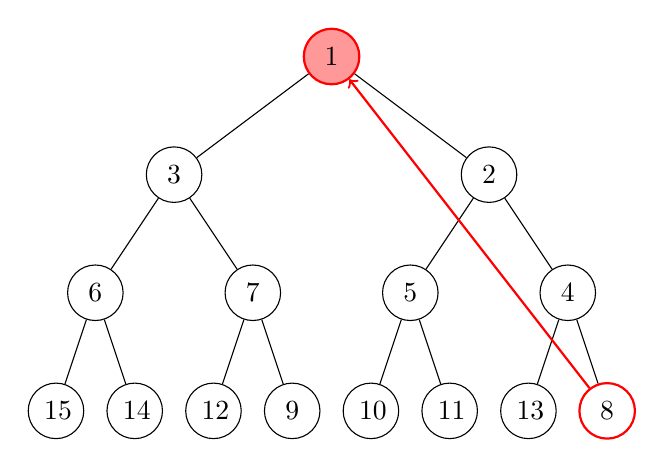
\begin{tikzpicture}[every node/.style={circle, draw=black, text width=0.3cm, align=center},
				   level 1/.style={sibling distance=40mm},
				   level 2/.style={sibling distance=20mm},
				   level 3/.style={sibling distance=10mm}]
\node[draw=red, thick, fill=red!40] (B) {1}
	child {node {3}
		child {node {6}
			child {node {15}}
			child {node {14}}
		}
		child {node {7}
			child {node {12}}
			child {node {9}}
		}
	}
	child {node {2}
		child {node {5}
			child {node {10}}
			child {node {11}}
		}
		child {node {4}
			child {node {13}}
			child {node[draw=red, thick] (A) {8}}
		}
	}
;

\draw[->, red, thick] (A) to (B);
\end{tikzpicture}
Får da dette resultatet. Og vi må nå flytte 8 ned til riktig posisjon.
\end{minipage}

\begin{minipage}{0.5\textwidth}
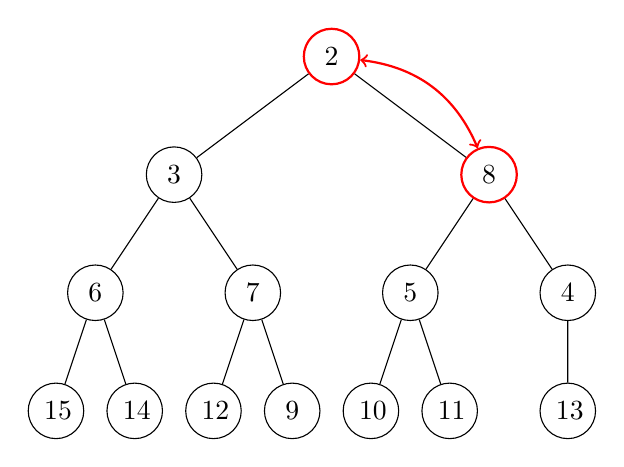
\begin{tikzpicture}[every node/.style={circle, draw=black, text width=0.3cm, align=center},
				   level 1/.style={sibling distance=40mm},
				   level 2/.style={sibling distance=20mm},
				   level 3/.style={sibling distance=10mm}]
\node[draw=red, thick](B){2}
	child {node {3}
		child {node {6}
			child {node {15}}
			child {node {14}}
		}
		child {node {7}
			child {node {12}}
			child {node {9}}
		}
	}
	child {node[draw=red, thick] (A) {8}
		child {node {5}
			child {node {10}}
			child {node {11}}
		}
		child {node {4}
			child {node {13}}
		}
	}
;
\draw[<->, red, thick] (A) to [bend right] (B);
\end{tikzpicture}
\end{minipage}
\begin{minipage}{0.5\textwidth}
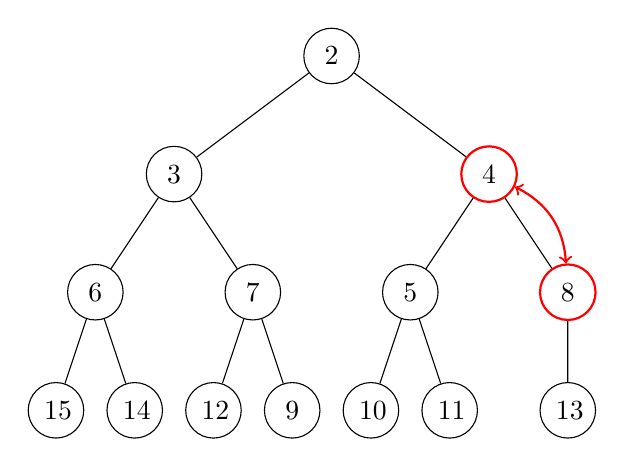
\begin{tikzpicture}[every node/.style={circle, draw=black, text width=0.3cm, align=center},
				   level 1/.style={sibling distance=40mm},
				   level 2/.style={sibling distance=20mm},
				   level 3/.style={sibling distance=10mm}]
\node{2}
	child {node {3}
		child {node {6}
			child {node {15}}
			child {node {14}}
		}
		child {node {7}
			child {node {12}}
			child {node {9}}
		}
	}
	child {node[draw=red, thick] (B) {4}
		child {node {5}
			child {node {10}}
			child {node {11}}
		}
		child {node[draw=red, thick] (A) {8}
			child {node {13}}
		}
	}
;
\draw[<->, red, thick] (A) to [bend right] (B);
\end{tikzpicture}
\end{minipage}

\newpage

%%% GRAFER %%%
\section{Grafer}

\begin{definition}
\emph{\textbf{Graf}}
En \textbf{graf} $\mathcal{G}$ består av en ikke-tom mengde noder $\mathcal{V}$ og en mengde kanter $\mathcal{E}$, slik at enhvet kant forbinder nøyaktig to noder med hverandre eller en node med seg selv.
\end{definition}

\subsection{Terminologi}
\begin{definition}
\emph{\textbf{Vektet}} En graf er vektet dersom hver kant har en tredje komponent. En verdi langs kanten.
\end{definition}
\begin{definition}
\emph{\textbf{Sti}} En sti gjennom grafen er en sekvens av noder $v_1, v_2, v_3, \dots, v_n$, slik at $(v_i,v_{i+1}) \in \mathcal{E}$ for $1 \leq i \leq n-1$.
\end{definition}
\begin{definition}
\emph{\textbf{Lengde}} Lengden til stien er lik antall kanter på stien.
\end{definition}
\begin{definition}
\emph{\textbf{Løkke}}  Ei løkke i en rettet graf er en vei med lengde $\geq 1$, slik at $v_1=v_n$. Løkken er \textit{enkel} dersom stien er enkel.
\end{definition}
\begin{definition}
\emph{\textbf{Asyklisk}}  En rettet graf er asyklisk dersom den ikke har noen løkker. DAG (Directed, Asyclic Graph).
\end{definition}
\begin{definition}
\emph{\textbf{Sammenhengende}} En urettet graf er sammenhengende dersom det fins en sti fra hver node til alle andre noder.
\end{definition}

\subsection{Topologisk sortering}
\begin{definition}
\emph{\textbf{Topologisk sortering}} En topologisk sortering (topologisk orden) av en rettet graf er en lineær ordning av nodene, slik at for hver rettet kant $\langle u,v \rangle$ fra node $u$ til node $v$, så kommer $u$ før $v$ i ordningen.
\end{definition}
\begin{figure}[h!]
\centering
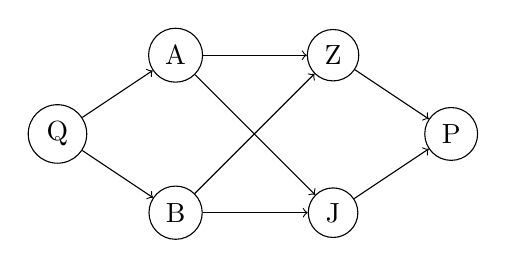
\begin{tikzpicture}[->]
\tikzstyle{vertex} = [circle, draw=black]
\tikzstyle{edge} = [draw=black]

\node[vertex] (A) at (1,0) {A};
\node[vertex] (Q) at (-0.5,-1) {Q};
\node[vertex] (B) at (1,-2) {B};
\node[vertex] (Z) at (3,0) {Z};
\node[vertex] (J) at (3,-2) {J};
\node[vertex] (P) at (4.5,-1) {P};

\draw[edge] (Q) -- (A);
\draw[edge] (Q) -- (B);
\draw[edge] (A) -- (Z);
\draw[edge] (A) -- (J);
\draw[edge] (B) -- (J);
\draw[edge] (B) -- (Z);
\draw[edge] (J) -- (P);
\draw[edge] (Z) -- (P);
\end{tikzpicture}
\caption{Eksempelfigur for topologisk sortering.}
\label{fig:graph}
\end{figure}

I figur \ref{fig:graph} har vi følgende lovlige topologiske sorteringer:

\begin{itemize}
\item
Q, A, B, J, Z, P
\item
Q, B, A, J, Z, P
\item
Q, A, B, Z, J, P
\item
Q, B, A, Z, J, P
\end{itemize}

\subsubsection{Algoritmer} De vanligste algoritmene for topologisk sortering har lineær kjøretid i antall noder, pluss antall kanter; O$(|\mathcal{V}|+|\mathcal{E}|)$. En av disse kommer det et eksempel på her.

\begin{Verbatim}[frame=single]
L <- empty list that will contain the sorted elements
S <- set of all nodes with no incoming edges

while S in non-empty do:
    remove a node n from S
    insert n into L
    for each node m with an edge e from n to m do:
        remove edge e from the graph
        if m had no other incoming edges then:
            insert m into S
if graph has edges then:
    return error (graph has at least one cycle)
else
    return L (a topofically sorted order)
\end{Verbatim}

\begin{lstlisting}[frame=none]
public List<E> topologicalSort (List<E> graph) {
	boolean[] visited = new boolean[graph.length];
	List<E> result = new ArrayList<>();

	for (int i = 0; i < graph.length; i++) {
		if (!visited[i])
			DFS(graph, visited, result, i);
	}
	return result;
}

public void DFS (List<E> graph, boolean[] visited, List<E> result, int i) {
	visited[i] = true;
	
	for (int v : graph[i]) {
		if (!visited[v])
			DFS(graph, visited, result, v);
	}
	result.add(i);
}
\end{lstlisting}
\vspace{-30pt}

\subsection{Dijkstra}
\begin{enumerate}
\item
For alle noder, sett avstanden fra startnoden $s$ lik $\infty$. Merk noden som \textit{ukjent}.
\item
Sett avstanden fra $s$ til seg selv lik 0.
\item
Velg en ukjent node $v$ med minimal avstand fra $s$ og marker $v$ som kjent.
\item
For hver ukjente nabonode $w$ til $v$: Dersom avstanden vi får ved å følge veien gjennom $v$, er kortere enn den gamle avstanden til $s$. Redusér avstanden til $s$ for $w$ og sett bakoverpekeren i $w$ til $v$.
\item
Akkurat som for uvektede grafer, ser vi bare etter potensielle forbedringer for naboer som ennå ikke er kjent.
\end{enumerate}

\begin{figure}[h!]
\centering
\scalebox{0.8}{
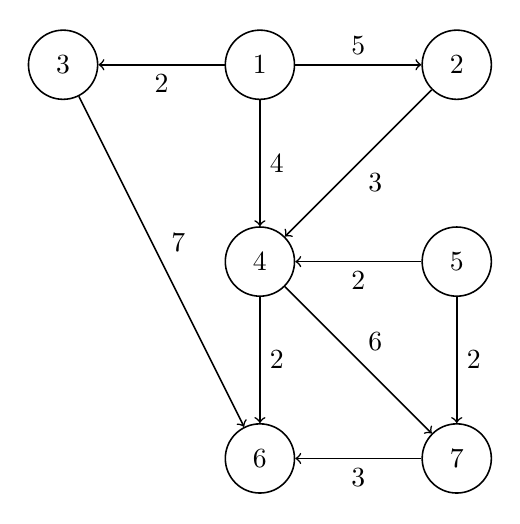
\begin{tikzpicture}[->,auto,node distance=2.5cm,line width=0.2mm]
\node[state] (A) {3};
\node[state] (B) [right of=A] {1};
\node[state] (C) [right of=B] {2};
\node[state] (D) [below of=B] {4};
\node[state] (E) [right of=D] {5};
\node[state] (F) [below of=D] {6};
\node[state] (G) [right of=F] {7}; 

\path 	(A) edge node {7} (F)
		(B) edge node {2} (A)
			edge node {4} (D)
			edge node {5} (C)
		(C) edge node {3} (D)
		(D) edge node {2} (F)
			edge node {6} (G)
		(E) edge node {2} (D)
			edge node {2} (G)
		(G) edge node {3} (F)
;
\end{tikzpicture}
}
\caption{Eksempelgraf for Dijkstra.}
\label{fig:graph2}
\end{figure}

\begin{table}
\centering
\begin{tabular}{c|ccc|ccc|ccc}
&&\textbf{Init}&&&\textbf{1}&&&\textbf{3}\\
V & known & dist. & from&known&dist.&from&known&dist.&from\\
\hline
1 & F & 0 & 0&T&0&0&T&0&0\\
2 & F & -- & 0&F&5&1&F&5&1\\
3 & F & -- & 0&F&2&1&T&2&1\\
4 & F & -- & 0&F&4&1&F&4&1\\
5 & F & -- & 0&F&--&0&F&--&0\\
6 & F & -- & 0&F&--&0&F&9&3\\
7 & F & -- & 0&F&--&0&F&--&0\\
\hline
\hline
&&\textbf{4}&&&\textbf{2}&&&\textbf{6}\\
V & known & dist. & from&known&dist.&from&known&dist.&from\\
\hline
1&T&0&0&T&0&0&T&0&0\\
2&F&5&1&T&5&1&T&5&1\\
3&T&2&1&T&2&1&T&2&1\\
4&T&4&1&T&4&1&T&4&1\\
5&F&--&0&F&--&0&F&--&0\\
6&F&6&4&F&6&4&T&6&4\\
7&F&10&4&F&10&4&F&10&4\\
\hline
\hline
&&\textbf{7}&\\
V & known & dist. & from\\
\cline{1-4}
1&T&0&0\\
2&T&5&1\\
3&T&2&1\\
4&T&4&1\\
5&F&--&0\\
6&T&6&4\\
7&T&10&4\\
\end{tabular}
\label{tab:dijkstra}
\caption{Tabell til Dikjstra-algoritmen på grafen i figur \ref{fig:graph2}.}
\end{table}


\paragraph{Algoritmen} Her er pseudokoden for Dijkstra.

\begin{Verbatim}[frame=single]
function Dijkstra (Graph, source):
    for each vertex v in Graph:
        distance[v] := infinity
        visited[v] := false;
        previous[v] := undefined;
    
    distance[source] = 0;
    insert source into Q;

    while Q is not empty:
        u := vertex in Q with smallest distance in distance[] 
                    and has not been visited;
        remove u from Q;
        visited[u] := true;

        for each neighbour v of u:
            alt := distance[u] + dist_between(u,v);
            if alt < dist[v];
                dist[v] := alt;
                previous[v] := u;
                if !visited[v]:
                    insert v into Q;
    return distance;
end function;
\end{Verbatim}
\newpage
\begin{lstlisting}[frame=none]
class Edge {
	final Vertex target;
	final double weight;
}

public void dijkstra (Vertex source) {
	source.minDistance = 0;
	PriorityQueue<Vertex> vertexQueue = new PriorityQueue<Vertex>();
	vertexQueue.add(source);

	while (!vertexQueue.isEmpty()) {
		Vertex u = vertexQueue.poll();
	
		for (Edge e : u.adjacencies) {
			Vertex v = e.target;
			double weight = e.weight;
			double distanceThroughU = u.minDistance + weight;
	
			if (distanceThroughU < v.minDistance) {
				vertexQueue.remove(v);
				v.minDistance = distanceThroughU;
				v.previous = u;
				vertexQueue.add(v);
			}
		}
	}
}
\end{lstlisting}

\subsection{Prim}
\begin{figure}[h!]
\centering
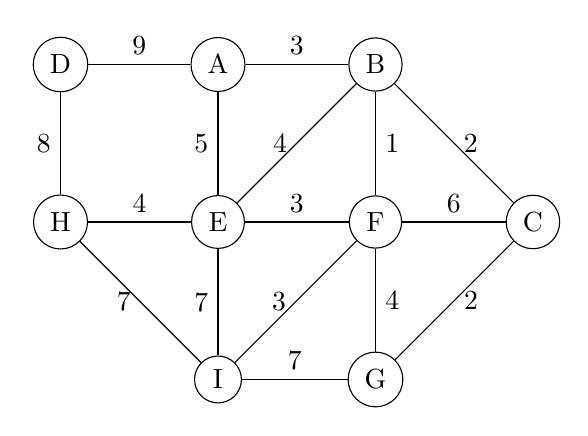
\begin{tikzpicture}
\tikzstyle{vertex} = [circle, draw=black]
\tikzstyle{edge} = [draw=black]
\tikzstyle{selected edge} = [-, red!100]

\node[vertex] (A) at (0,0) {A};
\node[vertex] (B) at (2,0) {B};
\node[vertex] (D) at (-2,0) {D};
\node[vertex] (C) at (4,-2) {C};
\node[vertex] (H) at (-2,-2) {H};
\node[vertex] (E) at (0,-2) {E};
\node[vertex] (F) at (2,-2) {F};
\node[vertex] (I) at (0,-4) {I};
\node[vertex] (G) at (2,-4) {G};

\path (A) edge node [above] {3} (B);
\path (A) edge node [left] {5} (E);
\path (A) edge node [above] {9} (D);
\path (B) edge node [right] {2} (C);
\path (B) edge node [right] {1} (F);
\path (B) edge node [left] {4} (E);
\path (C) edge node [above] {6} (F);
\path (C) edge node [right] {2} (G);
\path (D) edge node [left] {8} (H);
\path (E) edge node [above] {3} (F);
\path (E) edge node [left] {7} (I);
\path (F) edge node [right] {4} (G);
\path (F) edge node [left] {3} (I);
\path (G) edge node [above] {7} (I);
\path (H) edge node [left] {7} (I);
\path (H) edge node [above] {4} (E);
\end{tikzpicture}
\caption{Eksempelgraf for Prim og Kruskal.}
\label{fig:graph3}
\end{figure}

\subsubsection{Framgangsmåte}
\begin{enumerate}
\item
Initialiser et tre med en enkelt node, valgt tilfeldig fra grafen.
\item
Gro treet med én kant (av de kantene som går til en node som ikke er med i treet), finn den kanten med minst vekt og legg den inn i treet.
\item
Gjenta steg 2 til alle nodene er i treet.
\end{enumerate}

\begin{Verbatim}[frame=single]
PRIM(G, w, r) 
  for each u in G.V
    u.key = infinite
    u.parent = NIL
  r.key = 0
  Q = G.V
  while Q is not empty
    u = extract-min(Q)
    for each v in G.Adj[u]
      if (v in Q) and w(u,v) < v.key
        v.parent = u
        v.key = w(u,v)
\end{Verbatim}

Når man utfører Prims algoritme på grafen i figur \ref{fig:graph3}, så blir resultatet følgende:
\begin{figure}[h!]
\centering
\scalebox{0.8}{
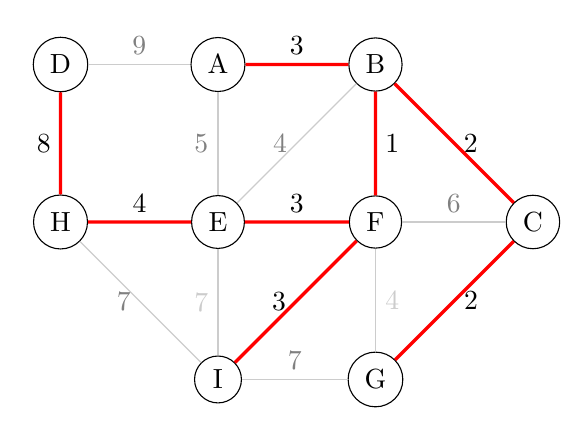
\begin{tikzpicture}
\tikzstyle{vertex} = [circle, draw=black]
\tikzstyle{edge} = [draw=black]
\tikzstyle{selected edge} = [-, red!100, very thick]

\node[vertex] (A) at (0,0) {A};
\node[vertex] (B) at (2,0) {B};
\node[vertex] (D) at (-2,0) {D};
\node[vertex] (C) at (4,-2) {C};
\node[vertex] (H) at (-2,-2) {H};
\node[vertex] (E) at (0,-2) {E};
\node[vertex] (F) at (2,-2) {F};
\node[vertex] (I) at (0,-4) {I};
\node[vertex] (G) at (2,-4) {G};

\path (A) edge node [above] {3} (B);
\path (A) edge[black!20] node [left, gray] {5} (E);
\path (A) edge[black!20] node [above, gray] {9} (D);
\path (B) edge node [right] {2} (C);
\path (B) edge node [right] {1} (F);
\path (B) edge[black!20] node [left, gray] {4} (E);
\path (C) edge[black!20] node [above, gray] {6} (F);
\path (C) edge node [right] {2} (G);
\path (D) edge node [left] {8} (H);
\path (E) edge node [above] {3} (F);
\path (E) edge[black!20] node [left] {7} (I);
\path (F) edge[black!20] node [right] {4} (G);
\path (F) edge node [left] {3} (I);
\path (G) edge[black!20] node [above, gray] {7} (I);
\path (H) edge[black!20] node [left, gray] {7} (I);
\path (H) edge node [above] {4} (E);

\draw[selected edge] (D) -- (H) -- (E) -- (F) -- (I) -- (F) -- (B) -- (A) -- (B) -- (C) -- (G);
\end{tikzpicture}
}
\caption{Eksempelgraf \ref{fig:graph3} etter Prims algoritme.}
\label{fig:prim}
\end{figure}

\begin{table}
\centering
\begin{tabular}{ccc}
&avs.&fra\\
A&0&--\\
B&3&A\\
C&2&B\\
D&8&H\\
E&3&F\\
F&1&B\\
G&2&C\\
H&4&E\\
I&3&F\\
\cline{2-2}
&26&\\
\cline{2-2}
\end{tabular}
\caption{Tabell for Prims algoritme på figur \ref{fig:prim}.}
\end{table}

\textbf{MERK:} løsningen i figur \ref{fig:prim} er \textit{ikke} unik. Eneste måten man kan få et unikt resultat er om alle vektene på kantene er unike. Det samme gjelder for Kruskal.

\newpage

\subsection{Kruskal}
\subsubsection{Framgangsmåte}
\begin{itemize}
\item
Lag en \textit{skog} $\mathcal{F}$ (en sett med trær), hver hver node i grafen er et separat tre.
\item
Lag et sett $\mathcal{S}$ som inneholder alle kantene til grafen.
\item
Så lenge $\mathcal{S}$ ikke er tom og $\mathcal{F}$ ikke ennå er et spanning-tre:
\begin{itemize}
\item
Fjern en kant men lavest vekt fra $\mathcal{S}$.
\item
Hvis kanten kobler to forskjellige trær, legg den i skogen slik at de to blir ett tre.
\end{itemize}
\end{itemize}
Når algoritmen er ferdig, så former skogen et minimum spanning-tre for grafen. 

\begin{Verbatim}[frame=single]
KRUSKAL (G):
  A = empty
  for each v in G.V:
    MAKE-SET(v)
  for each (u,v) ordered by weight(u,v), increasing:
    if FIND-SET(u) not in FIND-SET(v):
      A = A union {(u,v)}
      UNION(u,v)
  return A
\end{Verbatim}

\begin{figure}[h!]
\centering
\scalebox{0.8}{
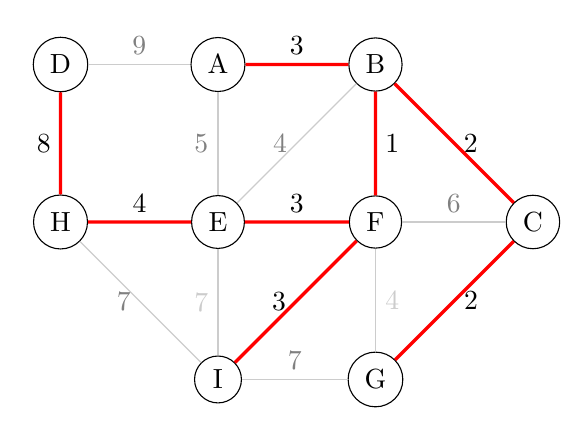
\begin{tikzpicture}
\tikzstyle{vertex} = [circle, draw=black]
\tikzstyle{edge} = [draw=black]
\tikzstyle{selected edge} = [-, red!100, very thick]

\node[vertex] (A) at (0,0) {A};
\node[vertex] (B) at (2,0) {B};
\node[vertex] (D) at (-2,0) {D};
\node[vertex] (C) at (4,-2) {C};
\node[vertex] (H) at (-2,-2) {H};
\node[vertex] (E) at (0,-2) {E};
\node[vertex] (F) at (2,-2) {F};
\node[vertex] (I) at (0,-4) {I};
\node[vertex] (G) at (2,-4) {G};

\path (A) edge node [above] {3} (B);
\path (A) edge[black!20] node [left, gray] {5} (E);
\path (A) edge[black!20] node [above, gray] {9} (D);
\path (B) edge node [right] {2} (C);
\path (B) edge node [right] {1} (F);
\path (B) edge[black!20] node [left, gray] {4} (E);
\path (C) edge[black!20] node [above, gray] {6} (F);
\path (C) edge node [right] {2} (G);
\path (D) edge node [left] {8} (H);
\path (E) edge node [above] {3} (F);
\path (E) edge[black!20] node [left] {7} (I);
\path (F) edge[black!20] node [right] {4} (G);
\path (F) edge node [left] {3} (I);
\path (G) edge[black!20] node [above, gray] {7} (I);
\path (H) edge[black!20] node [left, gray] {7} (I);
\path (H) edge node [above] {4} (E);

\draw[selected edge] (D) -- (H) -- (E) -- (F) -- (I) -- (F) -- (B) -- (A) -- (B) -- (C) -- (G);
\end{tikzpicture}
}
\caption{Eksempelgraf \ref{fig:graph3} etter Kruskals algoritme.}
\label{fig:kruskal}
\end{figure}

\begin{tabular}{r|ccccccccl}
\textbf{Kant} & FB&BC&CG&FI&FE&BA&EH&HD\\
\cline{1-9}
\textbf{Vekt}&1&2&2&3&3&3&4&8&$\Rightarrow$26
\end{tabular}

\newpage

% Dybde-først
\subsection{Dybde-først}
Dette er klassisk graf-traversering, generalisering av prefiks traversering for trær. Gitt start node $v$: rekursivt traverser alle nabonodene.
\begin{lstlisting}
public void depthFirstSearch(Node v)
	v.marked = true;
	for <each neighbour w to v>
		if (!w.marked)
			depthFirstSearch(w);
\end{lstlisting}

\begin{minipage}{0.5\textwidth}
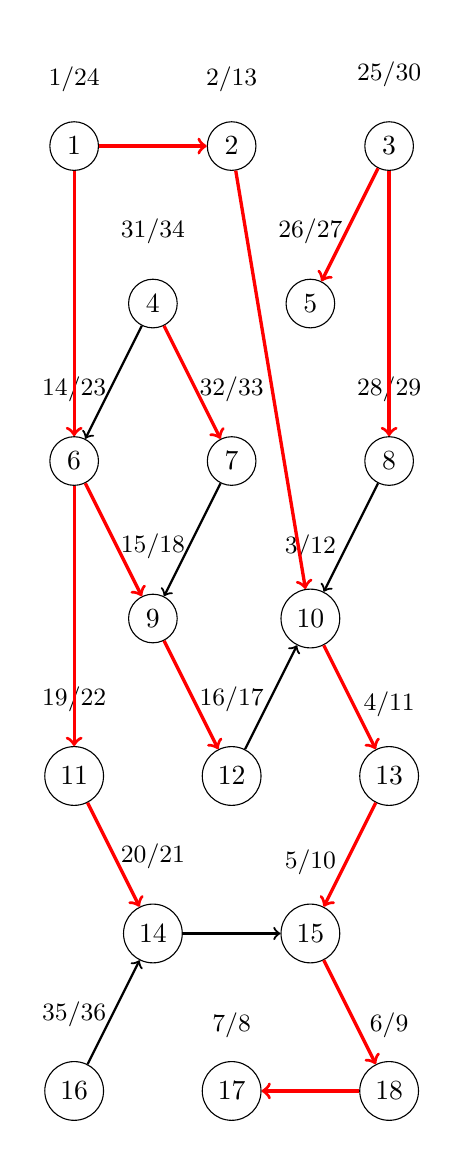
\begin{tikzpicture}[every node/.style={draw=black,circle}]
\node (1)[label={\small 1/24}] at (0,0) {1};
\node (2)[label={\small 2/13}] at (2,0) {2};
\node (3)[label={\small 25/30}] at (4,0) {3};
\node (4)[label={\small 31/34}] at (1,-2) {4};
\node (5)[label={\small 26/27}] at (3,-2) {5};
\node (6)[label={\small 14/23}] at (0,-4) {6};
\node (7)[label={\small 32/33}] at (2,-4) {7};
\node (8)[label={\small 28/29}] at (4,-4) {8};
\node (9)[label={\small 15/18}] at (1,-6) {9};
\node (10)[label={\small 3/12}] at (3,-6) {10};
\node (11)[label={\small 19/22}] at (0,-8) {11};
\node (12)[label={\small 16/17}] at (2,-8) {12};
\node (13)[label={\small 4/11}] at (4,-8) {13};
\node (14)[label={\small 20/21}] at (1,-10) {14};
\node (15)[label={\small 5/10}] at (3,-10) {15};
\node (16)[label={\small 35/36}] at (0,-12) {16};
\node (17)[label={\small 7/8}] at (2,-12) {17};
\node (18)[label={\small 6/9}] at (4,-12) {18};

\draw[->, very thick, red] (1) to (2);
\draw[->, very thick, red] (1) to (6);
\draw[->, very thick, red] (2) to (10);
\draw[->, very thick, red] (3) to (5);
\draw[->, very thick, red] (3) to (8);
\draw[->, thick] (4) to (6);
\draw[->, very thick, red] (4) to (7);
\draw[->, very thick, red] (6) to (9);
\draw[->, very thick, red] (6) to (11);
\draw[->, thick] (7) to (9);
\draw[->, thick] (8) to (10);
\draw[->, very thick, red] (9) to (12);
\draw[->, very thick, red] (10) to (13);
\draw[->, very thick, red] (11) to (14);
\draw[->, thick] (12) to (10);
\draw[->, very thick, red] (13) to (15);
\draw[->, thick] (14) to (15);
\draw[->, very thick, red] (15) to (18);
\draw[->, thick] (16) to (14);
\draw[->, very thick, red] (18) to (17);
\end{tikzpicture}
\end{minipage}
\begin{minipage}{0.5\textwidth}
Her gjør vi et depth-first search på grafen etter \textit{nodenes rekkefølge}. Tallene som står over hver node er starttid/sluttid.
\newline \newline
Første stien går over $1 \rightarrow 2 \rightarrow 10 \rightarrow 13 \rightarrow 15 \rightarrow 18 \rightarrow 17$, når vi kommer til 17, så er det ingen flere veier igjen å gå. Da noterer vi sluttiden og går tilbake på den samme stien, og finner at vi må helt tilbake til 1 for å finne en ny sti som tar oss videre. Da får vi stien: $1 \rightarrow 6 \rightarrow 9 \rightarrow 12$, fra 12 så går det en sti til 10. Men vi har allerede besøkt 10, så da må vi gå tilbake til 6 for å ta den andre stien derfra: $6 \rightarrow 11 \rightarrow 14$. Her må vi helt tilbake til 1 igjen, men alle stiene til 1 er tatt. Det samme for node 2, så vi må ta stiene fra node 3: $3 \rightarrow 5$ og $3 \rightarrow 8$. Så går vi vidre til 4: $4 \rightarrow 7$. Da står vi igjen med kun én ubesøkt node, som er 16. Så vi fører opp 16 til slutt, med besøktid 35 og sluttid 36.
\end{minipage}

\newpage

\subsection{Biconnectivity}
\theoremstyle{mytheoremstyle}
\newtheorem{biconnect}{Definisjon}[subsection]
\begin{biconnect}
En sammenhengende urettet graf er \textbf{bi-connected} hvis det ikke er noen noder som ved fjerning gjør at grafen blir usammenhengende. Slike noder heter cut-vertices eller articulation points.
\end{biconnect}

\begin{figure}[h!]
\centering
\scalebox{0.6}{
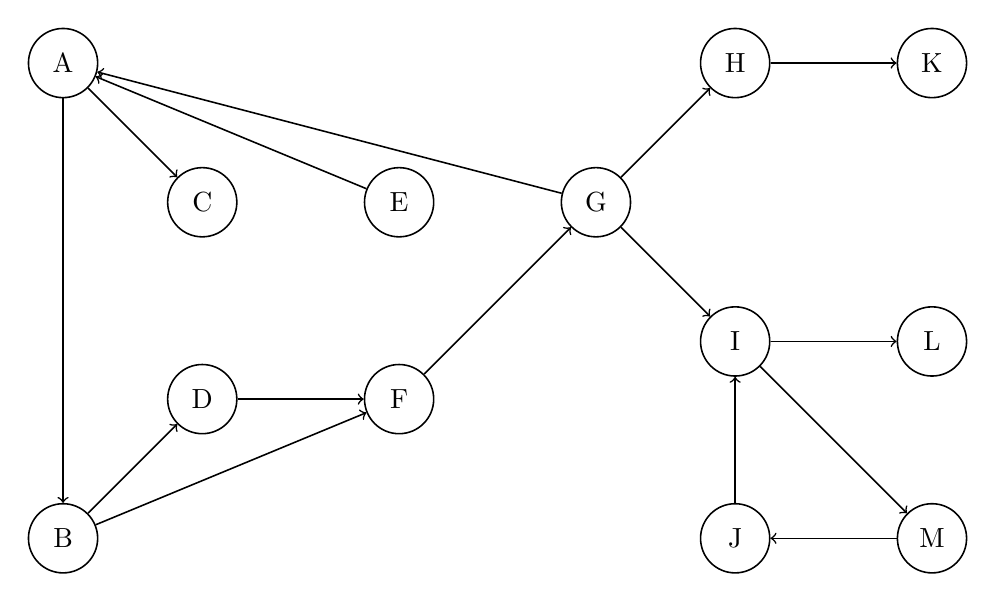
\begin{tikzpicture}[->,auto,node distance=2.5cm,line width=0.2mm]
\node[state] (A) {A};
\node[state] (C) [below right of=A] {C};
\node[state] (E) [right of=C] {E};
\node[state] (G) [right of=E] {G};
\node[state] (H) [above right of=G] {H};
\node[state] (K) [right of=H] {K};
\node[state] (D) [below of=C] {D};
\node[state] (F) [right of=D] {F};
\node[state] (I) [below right of=G] {I};
\node[state] (L) [right of=I] {L};
\node[state] (B) [below left of=D] {B};
\node[state] (J) [below of=I] {J};
\node[state] (M) [right of=J] {M};

\path 	(A) edge node {} (B)
			edge node {} (C)
		(B) edge node {} (D)
			edge node {} (F)
		(D) edge node {} (F)
		(E) edge node {} (A)
		(F) edge node {} (G)
		(G) edge node {} (I)
			edge node {} (H)
			edge node {} (A)
		(H) edge node {} (K)
		(I) edge node {} (L)
			edge node {} (M)
		(J) edge node {} (I)
		(M) edge node {} (J)
;
\end{tikzpicture}
}
\caption{Eksempelgraf for bi-connectivity.}
\label{fig:graphbi}
\end{figure}

Grafen i figur \ref{fig:graphbi} er \textit{ikke} bi-connected, fordi nodene A, I, G og H er articulation points.


\begin{figure}[h!]
\centering
\scalebox{0.6}{
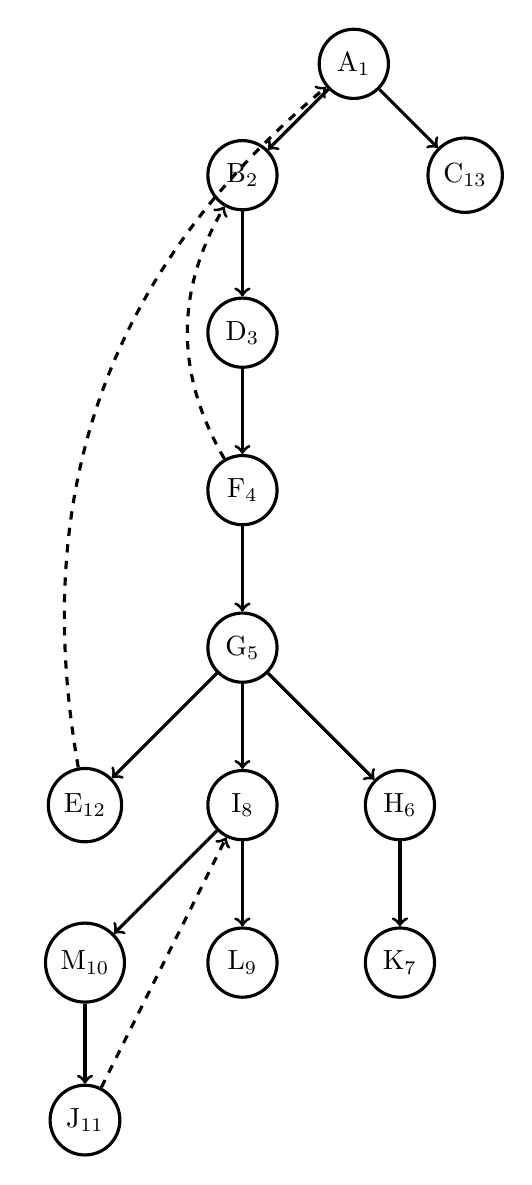
\begin{tikzpicture}[->,auto,node distance=2cm,line width=0.4mm]
\node[state] (A) {A$_1$};
\node[state] (B) [below left of=A] {B$_2$};
\node[state] (C) [below right of=A] {C$_{13}$};
\node[state] (D) [below of=B] {D$_3$};
\node[state] (F) [below of=D] {F$_4$};
\node[state] (G) [below of=F] {G$_5$};
\node[state] (I) [below of=G] {I$_8$};
\node[state] (E) [left of=I] {E$_{12}$};
\node[state] (H) [right of=I] {H$_6$};
\node[state] (L) [below of=I] {L$_9$};
\node[state] (M) [left of=L] {M$_{10}$};
\node[state] (K) [below of=H] {K$_7$};
\node[state] (J) [below of=M] {J$_{11}$};

\path (A) edge node {} (B)
		edge node {} (C)
	(B) edge node {} (D)
	(D) edge node {} (F)
	(F) edge node {} (G)
	(G) edge node {} (H)
		edge node {} (I)
		edge node {} (E)
	(I) edge node {} (M)
		edge node {} (L)
	(H) edge node {} (K)
	(M) edge node {} (J)
	(E) edge [bend left, dashed] node {} (A)
	(F) edge [bend left, dashed] node {} (B)
	(J) edge [dashed] node {} (I)
;
\end{tikzpicture}
}
\caption{DFS spenntre for grafen i figur \ref{fig:graphbi}.}
\label{fig:spanngraph}
\end{figure}

Når man går nedover kantene i grafen i figur \ref{fig:spanngraph}, så setter man kantene som \textit{\textbf{tree edges}}. Ubrukte kanter markeres som \textit{\textbf{back edges}}.

\newpage

\subsection{Strongly connected components (SCC)}
\theoremstyle{mytheoremstyle}
\newtheorem{scc}{Definisjon}[subsection]
\begin{scc}
Gitt en rettet graf $\mathcal{G} = (\mathcal{V}, \mathcal{E})$. En \textbf{strongly connected component} av $\mathcal{G}$ er et maksimalt sett av noder $U \subseteq \mathcal{V}$. For alle $u_1, u_2 \in U$ har vi at $u_1 \rightarrow^*u_2$ og $u_2\rightarrow^*u_1$.
\end{scc}

\begin{figure}[h!]
\centering
\scalebox{0.8}{
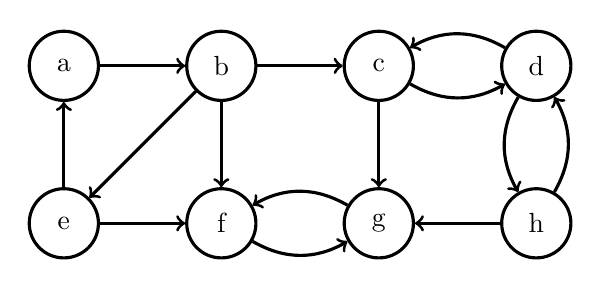
\begin{tikzpicture}[->,auto,node distance=2cm,line width=0.4mm]
  \node[state] 		(A)                    {a};
  \node[state]         	(B) [right of=A] {b};
  \node[state]		(C) [right of=B] {c};
  \node[state]		(D) [right of=C] {d};
  \node[state]		(E) [below of=A] {e};
  \node[state]		(F) [right of=E] {f};
  \node[state]		(G) [right of=F] {g};
  \node[state]		(H) [right of=G] {h};

  \path 	(A) edge node {} (B)
		(B) edge node {} (C)
		(B) edge node {} (F)
		(B) edge node {} (E)
		(C) edge [bend right] node {} (D)
		(C) edge node {} (G)
		(D) edge [bend right] node {} (C)
		(D) edge [bend right] node {} (H)
		(E) edge node {} (A)
		(E) edge node {} (F)
		(F) edge [bend right] node {} (G)
		(G) edge [bend right] node {} (F)
		(H) edge node {} (G)
		(H) edge [bend right] node {} (D);
\end{tikzpicture}
}
\caption{Eksempel på graf med noen SCCer.}
\label{fig:scc}
\end{figure}

Måten man finner ut om en graf har SCCer er:
\begin{enumerate}
\vspace{-15pt}
\item
Gjør en DFS på grafen. Nummerér nodene.
\item
Reverser grafen og gjør en DFS i \textit{\textbf{avtagende}} rekkefølge.
\vspace{-15pt}
\end{enumerate}
Man finner da gruppene med SCCer, det er grupper hvor alle nodene kan nå hverandre. I grafen i figur \ref{fig:scc} så er SCCene \{\{a, b, e\},\{f, g\},\{c, d, h\}\}.

\paragraph{DFS på graf i figur \ref{fig:scc}} Starter i \textit{a}, og setter start- og sluttid for nodene vi besøker.

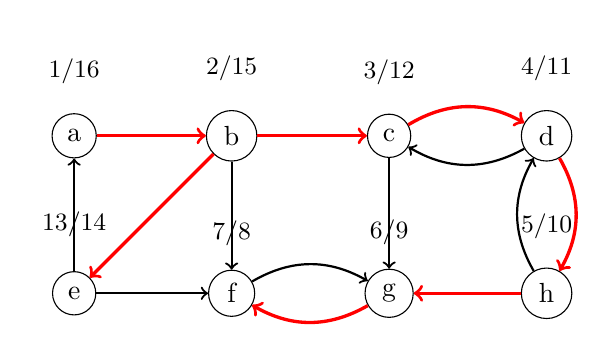
\begin{tikzpicture}[every node/.style={draw=black,circle}]
\node (a)[label={\small 1/16}] at (0,0) {a};
\node (b)[label={\small 2/15}] at (2,0) {b};
\node (c)[label={\small 3/12}] at (4,0) {c};
\node (d)[label={\small 4/11}] at (6,0) {d};
\node (e)[label={\small 13/14}] at (0,-2) {e};
\node (f)[label={\small 7/8}] at (2,-2) {f};
\node (g)[label={\small 6/9}] at (4,-2) {g};
\node (h)[label={\small 5/10}] at (6,-2) {h};

\draw[->, very thick, red] (a) to (b);
\draw[->, very thick, red] (b) to (c);
\draw[->, very thick, red] (c) to [bend left] (d);
\draw[->, thick] (d) to [bend left] (c);
\draw[->, very thick, red] (d) to [bend left] (h);
\draw[->, thick] (h) to [bend left] (d);
\draw[->, very thick, red] (h) to (g);
\draw[->, thick] (c) to (g);
\draw[->, very thick, red] (g) to [bend left] (f);
\draw[->, thick] (f) to [bend left] (g);
\draw[->, thick] (b) to (f);
\draw[->, thick] (e) to (f);
\draw[->, very thick, red] (b) to (e);
\draw[->, thick] (e) to (a);
\end{tikzpicture}

Reverserer kantene og tar en ny DFS i avtagende rekkefølge:

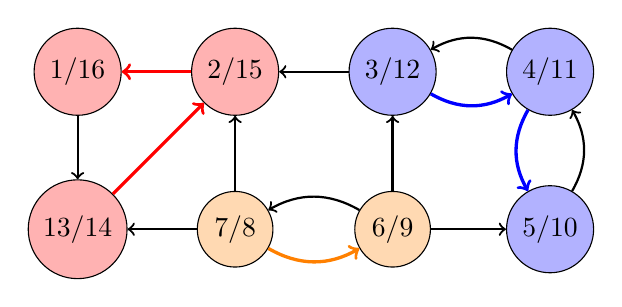
\begin{tikzpicture}[every node/.style={draw=black,circle}]
\node[fill=red!30] (a) at (0,0) {1/16};
\node[fill=red!30] (b) at (2,0) {2/15};
\node[fill=blue!30] (c) at (4,0) {3/12};
\node[fill=blue!30] (d) at (6,0) {4/11};
\node[fill=red!30] (e) at (0,-2) {13/14};
\node[fill=orange!30] (f) at (2,-2) {7/8};
\node[fill=orange!30] (g) at (4,-2) {6/9};
\node[fill=blue!30] (h) at (6,-2) {5/10};

\draw[<-, very thick, red] (a) to (b);
\draw[<-, thick] (b) to (c);
\draw[<-, thick] (c) to [bend left] (d);
\draw[<-, very thick, blue] (d) to [bend left] (c);
\draw[<-, thick] (d) to [bend left] (h);
\draw[<-, very thick, blue] (h) to [bend left] (d);
\draw[<-, thick] (h) to (g);
\draw[<-, thick] (c) to (g);
\draw[<-, very thick, orange] (g) to [bend left] (f);
\draw[<-, thick] (f) to [bend left] (g);
\draw[<-, thick] (b) to (f);
\draw[<-, thick] (e) to (f);
\draw[<-, very thick, red] (b) to (e);
\draw[<-, thick] (e) to (a);
\end{tikzpicture}

Da finner vi SCCene som nevnt over.

\newpage

%%% KOMBINATORISK SØK %%%
\section{Kombinatorisk søk}
Kombinatorisk søk-algoritmer er ofte problemer som er NP-hard. Men problemene kan løses effektivt om de brytes ned. Et eksempel på et problem hvor man får bruk for kombinatorisk søk er å plassere åtte dronninger på et sjakkbrett. 
\vspace{-10pt}
\subsection{Permutasjoner}

En permutasjon er å rearrangere objekter. For eksempel så fins det seks permutasjoner av settet \{1,2,3\}, som er: (1,2,3), (1,3,2), (2,1,3), (2,3,1), (3,1,2) og (3,2,1).
\vspace{-20pt}
\paragraph{Alle mulige permutasjoner av tallene fra 0 til $n-1$}.
\begin{lstlisting}[frame=none]
class Gen {
	int[] p; int n;
	boolean[] used;
	
	Gen (int i) {
		n = i; p = new int[n];
		used = new boolean[n];
	
		for (int j = 0; j < n; j++) {
			used[j] = false;
		}
	}

	void gen(int place) {
		for (int number = 0; number < n; number++) {
			if (!used[number]) {
				used[number] = true;
				p[place] = number;
				
				if (place < n-1) { gen(place+1); }
				else { <deliver p to further use.> }
				used[number] = false;
\end{lstlisting}
\vspace{-30pt}
%%% TEKSTALGORITMER %%%
\section{Tekstalgoritmer}

% Brute force
\subsection{Brute force}
Brute force metoden sjekker en og en karakter i teksten med nålen, og flytter med 1 om det er mismatch.

\subsubsection{Analyse}
Worst case så får vi mismatch $(n-m)$ ganger og suksess $(n-m)+1$ ganger. Totale sammenligninger er $((n-m)+1 \times m)$ som gir kjøretid O($n^2$).

% Boyer Moore
\subsection{Boyer Moore}
\begin{itemize}
\item
Først må man lage «bad match table».
\item
Sammenligne nålen med teksten, starter med karakteren lengst til høyre i nålen.
\item
Hvis mismatch, flytt nålen fram iht. verdien i tabellen.
\end{itemize}

\subsubsection{Eksempel: Bad character shift}
\begin{description}
\item[Pattern (nål)] tooth
\item[Tekst] trusthardtoothbrushes
\end{description}

\paragraph{1.} Konstruere «bad match table». 
\begin{center}
\texttt{value = length - index - 1}
\end{center}
Alle andre bokstaver har verdi lik lengden.
\begin{center}
\begin{tabular}{rccccc}
&T&O&O&T&H\\
index:&0&1&2&3&4\\
\end{tabular}
\end{center}
Lengden på denne nålen er 5. Finner verdiene ved å bruke \texttt{value = length - index - 1}.
\begin{center}
\begin{tabular}{cccl}
T = & $5-0-1$&= 4\\
O = & $5-1-1$&= 3\\
O = & $5-1-2$&= 2&Erstatter her forrige verdi av O med ny verdi til O.\\
T = &$5-3-1$& = 1&Erstatter her forrige verdi av T med ny verdi til T.\\
H = &5 &&Verdien skal ikke være mindre enn 1. Får da verdi lik lengden.\\
\end{tabular}

\begin{tabular}{l|llll}
Bokstav&T&O&H&$*$\\
\hline
Verdi&1&2&5&5\\
\end{tabular}
\end{center}

\scalebox{0.9}{
\begin{tabular}{cccccccccccccccccccccc}
&T&R&U&S&\textcolor{red}{T}&\textcolor{red}{H}&A&R&D&T&\textcolor{red}{O}&O&\textcolor{red}{T}&H&B&R&U&S&H&E&S\\
\textbf{1.}&T&O&O&T&\textcolor{red}{H}\\
\textbf{2.}&&T&O&\textcolor{red}{O}&\textcolor{dkgreen}{T}&\textcolor{dkgreen}{H}\\
\textbf{3.}&&&&&&&T&O&O&T&\textcolor{red}{H}\\
\textbf{4.}&&&&&&&&&T&O&O&T&\textcolor{red}{H}\\
\textbf{5.}&&&&&&&&&&\textcolor{dkgreen}{T}&\textcolor{dkgreen}{O}&\textcolor{dkgreen}{O}&\textcolor{dkgreen}{T}&\textcolor{dkgreen}{H}\\
\end{tabular}
}

I steg \textbf{1.} får vi mismatch på H, fordi den ikke er det samme som T. Da må vi slå opp i tabellen på den bokstaven som \textbf{\textit{vi møter i teksten}}, og hoppe fram tilsvarende antall steg. I første tilfellet skal vi hoppe 1 plass fram (for 1 er verdien til T). 

Sjekker på nytt i steg \textbf{2.}, her får vi match på T og H, men mismatch på O. Da hopper vi S-plasser frem. Siden S ikke er med i tabellen vår (eller den er med som $*$, som er alle andre bokstaver), så hopper vi 5 plasser frem.

I steg \textbf{3.} får vi mismatch på H mot O, og må hoppe O-plasser frem---altså 2. I steg \textbf{4.} er det mismatch mellom H og T, vi hopper T-plasser frem---altså 1. Og vips! Så har vi funnet nålen i teksten vår!

\paragraph{Analyse}
Worst case er det samme som brute force. Input tekst $1^n$ kjører $n$ ganger, og nål $011\dots1$ kjører $m$ ganger. Dette gir O($nm$). Best case har input tekst $1^n$ og nål $0^m$, som gir O($n/m$). Average case er O($m/|\Sigma|$), raskere enn brute force.


\subsubsection{Eksempel: Good suffix shift}
Konstruere \textit{good suffix table} for nålen \texttt{TCCTATTCTT}.

\begin{minipage}{0.5\textwidth}
\paragraph{1.} Sjekker først \textit{ikke}-\texttt{T}, det er to shift før man finner dette.
\\
\noindent\texttt{TCCTATTCT\textcolor{red}{T}}\\
\texttt{--TCCTATT\textcolor{red}{C}TT}
\\
\paragraph{2.} Så sjekker man \textit{ikke}-\texttt{TT}. Dette finner man etter ett shift.
\\
\noindent\texttt{TCCTATTC\textcolor{red}{TT}}\\
\texttt{-TCCTATT\textcolor{red}{CT}T}
\\
\paragraph{3.} For å finne \textit{ikke}-\texttt{CTT} må vi flytte 3 steg; til \texttt{ATT}.
\\
\noindent\texttt{TCCTATT\textcolor{red}{CTT}}\\
\texttt{---TCCT\textcolor{red}{ATT}CTT}
\end{minipage}
\hspace{10pt}
\begin{minipage}{0.5\textwidth}
\paragraph{4.} Så kommer vi til \textit{ikke}-\texttt{TCTT}. Denne eksisterer ikke, MEN om nålen har lik suffix som prefiks (her \texttt{T} som start og slutt), så flytter vi bare fram til prefiksen. Da må vi flytte nålen 9 hakk, selv om lengden er 10.
\\
\noindent\texttt{TCCTATTCT\textcolor{red}{T}}\\
\texttt{---------\textcolor{red}{T}CCTATTCTT}
\\
Alle de neste shiftene vil også være dette, fordi de får ingen andre treff i nålen.
\end{minipage}

\vspace{10pt}

\noindent Vi får da følgende good suffix table:
\begin{table}[h!]
\centering
\begin{tabular}{crc}
index&mismatch&shift\\
\hline
0&\texttt{\textcolor{red}{T}}&2\\
1&\texttt{\textcolor{red}{T}T}&1\\
2&\texttt{\textcolor{red}{C}TT}&3\\
3&\texttt{\textcolor{red}{T}CTT}&9\\
4&\texttt{\textcolor{red}{T}TCTT}&9\\
5&\texttt{\textcolor{red}{A}TTCTT}&9\\
6&\texttt{\textcolor{red}{T}ATTCTT}&9\\
7&\texttt{\textcolor{red}{C}TATTCTT}&9\\
8&\texttt{\textcolor{red}{C}CTATTCTT}&9\\
9&\texttt{\textcolor{red}{T}CCTATTCTT}&9\\
\end{tabular}
\caption{Eksempel på good suffix table.}
\label{tab:gst}
\end{table}

\newpage
\subsection{Huffman}
\paragraph{Regler}
\begin{enumerate}
\item
Hvert tegn som forekommer i teksten skal ha sin egen entydige kode.
\item
Ingen kode er prefiks i en annen kode.
\end{enumerate}

\paragraph{Algoritme}
\begin{itemize}
\item
Lag en \textit{frekvenstabell} for alle tegn som forekommer i teksten.
\item
Betrakt hvert tegn som en node, og legg dem inn en prioritetskø P med frekvensen som vekt.
\item
Mens P har mer enn ett element:
\begin{itemize}
\item
Ta ut de to minste nodene fra P.
\item
Gi dem en felles foreldrenode med vekt lik summen av de to nodenes vekter.
\item
Legg foreldrenoden inn i P.
\end{itemize}
\item
Huffmankoden til et tegn (løvnode) får vi ved å gå fra roten og gi en '0' når vi går til venste og '1' når vi går til høyre.
\item
Resultatfilen består av to deler: en tabell over Huffmankoder med tilhørende tegn og den Huffmankodede datafilen.
\end{itemize}

\subsubsection{Eksempel på Huffmankoding}
\begin{table}[h!]
\centering
\begin{tabular}{ccc}
Karakter&Kode&Frekvens\\
\hline
n&11&4\\
c&01&3\\
o&101&2\\
r&100&2\\
e&001&2\\
u&000&1\\
\end{tabular}
\caption{Eksempel på en Huffmantabell.}
\label{tab:huffman}
\end{table}

\begin{figure}[h!]
\centering
\begin{tikzpicture}[every node/.style={inner sep=3pt},
				   level 1/.style={sibling distance=30mm},
				   level 2/.style={sibling distance=20mm},
				   level 3/.style={sibling distance=15mm}]

\node[circle]{14}
	child {node[circle] {6} 
		child {node[circle] {3} 
			child {node[circle split] {u \nodepart{lower} 1} }
			child {node[circle split] {e \nodepart{lower} 2} }
		}
		child {node[circle split] {c \nodepart{lower} 3} }
	}
	child {node[circle] {8} 
		child {node[circle] {4} 
			child {node[circle split] {r \nodepart{lower} 2} }
			child {node[circle split] {o \nodepart{lower} 2} }
		}
	child {node[circle split] {n \nodepart{lower} 4} }
	}
;

\end{tikzpicture}
\label{fig:huffman}
\caption{Huffmantreet for tabellen i tabell \ref{tab:huffman}.}
\end{figure}



%%% SORTERING %%%
\section{Sortering}


\begin{table}
\centering
\begin{tabular}{l|lll|l}
&\textbf{Tid}&&&\textbf{Rom}\\
\textbf{Algoritme}&Best&Average&Worst&Worst\\
\hline
Quicksort&
\textcolor{orange}{O$(\log (n))$}&\textcolor{dkgreen}{O$(\log (n))$}&\textcolor{red}{O$(n^2)$}&\textcolor{orange}{O$(n)$}\\
Mergesort&
\textcolor{orange}{O$(\log (n))$}&\textcolor{dkgreen}{O$(\log (n))$}&\textcolor{dkgreen}{O$(\log (n))$}&\textcolor{dkgreen}{O$(1)$}\\
Heapsort&
\textcolor{orange}{O$(\log (n))$}&\textcolor{dkgreen}{O$(\log (n))$}&\textcolor{dkgreen}{O$(\log (n))$}&\textcolor{dkgreen}{O$(n)$}\\
Bubble sort&
\textcolor{dkgreen}{O$(n)$}&\textcolor{red}{O$(n^2)$}&\textcolor{red}{O$(n^2)$}&\textcolor{dkgreen}{O$(n)$}\\
Insertion sort&
\textcolor{dkgreen}{O$(n)$}&\textcolor{red}{O$(n^2)$}&\textcolor{red}{O$(n^2)$}&\textcolor{dkgreen}{O$(1)$}\\
Selection sort&
\textcolor{red}{O$(n^2)$}&\textcolor{red}{O$(n^2)$}&\textcolor{red}{O$(n^2)$}&\textcolor{dkgreen}{O$(1)$}\\
Bucket sort&
\textcolor{dkgreen}{O$(n+k)$}&\textcolor{dkgreen}{O$(n+k)$}&\textcolor{red}{O$(n^2)$}&\textcolor{orange}{O$(nk)$}\\
Radix sort&
\textcolor{dkgreen}{O$(nk)$}&\textcolor{dkgreen}{O$(nk)$}&\textcolor{dkgreen}{O$(nk)$}&\textcolor{orange}{O$(n+k)$}\\
\end{tabular}
\label{tab:sorting}
\caption{Kompleksiteten til forskjellige sorteringsalgoritmer.}
\end{table}

\subsection{Quicksort}
Quicksort er en \textit{divide and conquer} algoritme. Den deler først en stor array inn i to mindre sub-arrayer: de mindre og de større verdiene. Sorterer så sub-arrayene rekursivt.

\begin{enumerate}
\item
Velg et element, kalt \textit{pivot}, fra arrayen.
\item
Reorder arrayen slik at alle elementene med vardier mindre enn pivot kommer før pivot, og alle elementer større enn pivot kommer etter. Pivot er på sin sluttplass. Dette kalles \textit{partisjonering}.
\item
Rekursivt gjenta stegene over på sub-arrayene med mindre og større verdier.
\end{enumerate}

\begin{Verbatim}[frame=single]
quicksort(A, i, k):
    if i < k:
        p := partition(A, i, k)
        quicksort(A, i, p-1)
        quicksort(A, p+1, k)

partition(array, left, right)
    pivotIndex := choosePivot(array, left, right)
    pivotValue := array[pivotIndex]
    swap array[pivotIndex] and array[right]
    storeIndex := left
    for i from left to right - 1
        if array[i] < pivotValue
            swap array[i] and array[storeIndex]
            storeIndex := storeIndex+1
    swap array[storeIndex] and array[right]
    return storeIndex
\end{Verbatim}

\subsection{Mergesort}
Mergesort er en \textit{divide and conquer} algoritme.
\begin{enumerate}
\item
Del den usorterte listen i \textit{n} sublister, hvor hver inneholder \textit{ett} element.
\item
Smelt sammen sublistene for å lage nye sorterte sublister til det er bare ei liste igjen. Dette er den sorterte listen.
\end{enumerate}

\subsection{Heapsort}
Heapsort er en \textit{in-place} algoritme, men den er ikke en \textit{stable sort}.

Først bygger man en heap ut av dataene. Ofte plassert i en array etter kravene for et komplett binært tre. Roten er lagret på index 0, hvis \texttt{i} er indeksen til \textit{denne} noden, så:\vspace{-10pt}
\begin{Verbatim}
iParent     = floot((i-1)/2)
iLeftChild  = 2*i+1
iRightChild = 2*i+2
\end{Verbatim}

I det andre steget lager man en sortert array ved gjentatte ganger fjerne største element fra heapen (roten), og sette det inn i arrayen. Heapen er oppdatert etter hver sletting, for å opprettholde kravene. Når alle elementene er slettet fra heapen, er resultatet en sortert array.

\subsection{Bubble sort}
Bubble sort, også kalt sinking sort, er en sammenlignings-sorteringsalgoritme. Den er for treig for all praktisk bruk, til og med treigere enn insertion sort.

\begin{Verbatim}[frame=single]
bubblesort(A : list of sortable items)
    n = length(A)
    do:
        swapped = false
        for i = 1 to n-1 inclusive do
            if A[i-1] > A[i] then
               swap(A[i-1], A[i])
               swapped = true
    while not swapped
\end{Verbatim}

\subsection{Insertion sort}
Enkel sorteringsalgoritme, som ikke er særlig effektiv på større lister. Da er algoritmer som quicksort, heapsort osv å foretrekke.

\begin{Verbatim}[frame=single]
for i = 1 to length (A)
    x = A[i]
    j = i
    while j > 0 and A[j-1] > x
        A[j] = A[j-1]
        j = j-1
    A[j] = x
\end{Verbatim}

\subsection{Selection sort}
Selection sort er en \textit{in-place} sammenlignings-algoritme.

\noindent La $\mathcal{L}$ være et ikke-tomt sett og $f : \mathcal{L} \rightarrow \mathcal{L}$, slik at $f(\mathcal{L}) = \mathcal{L}'$ hvor:
\begin{enumerate}
\item
$\mathcal{L}'$ er en permutasjon av $\mathcal{L}$,

\item
$e_i \leq e_{i+1}$ for alle $e \in \mathcal{L}'$ og $i \in \mathbb{N}$,

\item
$f(\mathcal{L}) = \left\{\begin{array}{ll}
   \mathcal{L} & if |\mathcal{L}|=1\\
    \{s\} \cup f(\mathcal{L}_s),&\mathrm{ellers}
  \end{array}\right.$

\item
$s$ er det \textit{minste elementet} i $\mathcal{L}$, og

\item
$\mathcal{L}_s$ er settet med elementer av $\mathcal{L}$ uten instansen av det minste elementet fra $\mathcal{L}$.
\end{enumerate}

Algoritmen finner minste verdi, bytter denne med verdien i første posisjon, og repeterer disse stegene for resten av listen. 

\subsection{Bucket sort}
Bucket sort, eller bin sort, er en \textit{distribution sort} algoritme.

\begin{enumerate}
\item
Sett opp en array med tomme «bøtter».
\item
\textbf{Scatter}: gå over den orginale arrayen, og putt hvert objekt i sin bøtte.
\item
Sortert hver ikke-tomme bøtte.
\item
\textbf{Gather}: besøk alle bøttene etter orden, og putt alle elementer tilbake i den orginale arrayen.
\end{enumerate}

\begin{Verbatim}[frame=single]
function bucketSort(array, n)
    buckets <- new array of n empty lists
    for i = 0 to (length(array) - 1) do
        insert array[i] into buckets[mbits(array[i], k)]
    for i = 0 to n - 1 do
        nextSort(buckets[i]);
    return the concatenation of buckets[0],...,buckets[n-1]
\end{Verbatim}

\subsection{Radix sort}
Radix sort er en \textit{non-comparative} integer sorterings algoritme. Er i samme familie som bucket sort.

\begin{enumerate}
\item
Ta det minst signifikante tallet av hver nøkkel.
\item
Gruppér nøklene basert på dette tallet.
\item
Gjenta til grupperingsprosessen med hvert høyere signifikante bit.
\end{enumerate}

\paragraph{Eksempel} Orginal, usortert lise: 170, 45, 75, 90, 802, 2, 24, 66
\begin{itemize}
\item
Sortere på minst signifikante (1-er plassen): 17\textcolor{red}{0}, 9\textcolor{red}{0}, 80\textcolor{red}{2}, \textcolor{red}{2}, 2\textcolor{red}{4}, 4\textcolor{red}{5}, 7\textcolor{red}{5}, 6\textcolor{red}{6}
\item
Sortere på 10-er plassen: 8\textcolor{red}{0}2, 2, \textcolor{red}{2}4, \textcolor{red}{4}5, \textcolor{red}{6}6, 1\textcolor{red}{7}0, \textcolor{red}{7}5, \textcolor{red}{9}0
\item
Sortere på 100 plassen: 2, 24, 45, 66, 75, 90, \textcolor{red}{1}70, \textcolor{red}{8}02
\end{itemize}

\newpage

\section{Gamle eksamensoppgaver}
Ved å gå gjennom alle gamle eksamensoppgaver (fra 2009 til 2013) og notere hvor mange poeng hver «pensum kategori» teller, så har jeg kommet fram til følgende skjema:

\includegraphics[width=\textwidth]{stats.pdf}

Det er helt klart binære trær, grafer, tekstalgoritmer, sortering og implementasjonsoppgaver som dominerer. I denne seksjonen skal jeg svare på noen eksamensoppgaver.

\subsection{Tekstalgoritmer (oppgave 7, H2011)}
\paragraph{7a) Beregn \textit{good suffix shift} av nålen: \texttt{a b c a b c a c a b}}
I indeks 1, så ser vi at ikke-\texttt{a b} ikke eksisterer i nåla, dermed må vi flytte lik lengden av nåla som er 10. I indeks 2 finner vi at nålens prefiks \texttt{a b} er lik nålens suffix. For mismatch etter denne trenger vi ikke shifte lenger enn til når prefiks og suffix er justert til hverandre, altså shifte 8.
\begin{center}
\begin{tabular}{crc}
indeks & mismatch & shift\\
\hline
0&\textcolor{red}{b}&1\\
1&\textcolor{red}{a}b&10\\
2&\textcolor{red}{c}ab&8\\
3&\textcolor{red}{a}cab&5\\
4&\textcolor{red}{c}acab&8\\
5&\textcolor{red}{b}cacab&8\\
6&\textcolor{red}{a}bcacab&8\\
7&\textcolor{red}{c}abcacab&8\\
8&\textcolor{red}{b}cabcacab&8\\
9&\textcolor{red}{a}bcabcacab&8\\
\end{tabular}
\end{center}

\newpage

\paragraph{7b) En mismatch er funnet under leting etter nålen \texttt{a b c a b c a c a b} som angitt nedenfor:\vspace{-20pt}}
\begin{Verbatim}
Høystakk: a a c a b c a a b c a b c a b c a c a b
     Nål: a b c a b c a c a b
\end{Verbatim}
\vspace{-30pt}
\paragraph{Hvor i høystakken vil \textit{Boyer Moore}-algoritmen lete etter neste match? (dvs. hvor langt vil Boyer Moore skifte nålen etter denne mismatch?)}
Med Boyer Moore bad character shift vil den gøre et shift på 2 for å lete etter neste match. Shift-tabellen må konstrueres:

\begin{tabular}{cccc}
\texttt{a}&\texttt{b}&\texttt{c}&\texttt{*}\\
\hline
1&5&2&10
\end{tabular}

\noindent Hvor \texttt{*} er alle andre karakterer enn \texttt{a}, \texttt{b} eller \texttt{c}. Og verdien er \texttt{value = length - index - 1}. Hvor length er lengden av nåla = 10. Og indeks er karakterens indeks i nåla:

\begin{tabular}{rcccccccccc}
Karakter&a&b&c&a&b&c&a&c&a&b\\
Indeks&0&1&2&3&4&5&6&7&8&9\\
\end{tabular}

\noindent Verdien i shift-tabellen skal være lavest mulig, men kan ikke være mindre enn 1. For \texttt{a}, \texttt{b} og \texttt{c} blir det:

\begin{tabular}{ccc}
\texttt{a}&$10-8-1$&$=1$\\
\texttt{b}&$10-4-1$&$=5$\\
\texttt{c}&$10-7-1$&$=2$\\
\end{tabular}

\noindent I oppgaven er det mismatch på \texttt{c} i høystakken. Og siden shift-verdien til \texttt{c} er 2, så flyttes nåla 2 nedover høystakken for neste match.

\begin{Verbatim}
Høystakk: a a c a b c a a b c a b c a b c a c a b
     Nål: a b c a b c a c a b
   Shift: . . a b c a b c a c a b
\end{Verbatim}

\newpage

\paragraph{7c) Lag en Huffmankode for strengen \texttt{nonconcurrence}. Vis dekodingstabellen.}
Koden er ikke unik. For at koden skal være unik, så må karakterenes frekvens også være unik. Et eksempel kan være at \texttt{u} og \texttt{o} er naboer istedenfor \texttt{u} og \texttt{e}, da ville \texttt{o} hatt koden 001, og ikke 101.

Huffmanntreet bygges ved å sette sammen de to og to laveste frekvensene til en ny frekvens-forelder. Dette gjør at den karakteren med høyst frekvens får korteste kode. Kantene til høyre telles som '1', og kantene til venstre som '0'.

\begin{minipage}{0.5\textwidth}
\begin{tabular}{crc}
Karakter&Kode&Frekvens\\
\hline
n&11&4\\
c&01&3\\
o&101&2\\
r&100&2\\
e&001&2\\
u&000&1\\
\end{tabular}
\end{minipage}
\begin{minipage}{0.5\textwidth}
\vspace{20pt}
\begin{tikzpicture}[level distance=10mm, level 1/.style={sibling distance=30mm}, level 2/.style={sibling distance=15mm}]
\node{14}
	child { node {6} 
		child { node {3} 
			child { node[rectangle split, below] { u \nodepart{two} 1} }
			child { node[rectangle split, below] { e \nodepart{two} 2} }
		}
		child { node[rectangle split, below] { c \nodepart{two} 3} }
	}
	child { node {8} 
		child { node {4} 
			child { node[rectangle split, below] { r \nodepart{two} 2} }
			child { node[rectangle split, below] { o \nodepart{two} 2} }
		}
		child { node[rectangle split, below] { n \nodepart{two} 4} }		
	}
;
\end{tikzpicture}
\end{minipage}

\subsection{Binære søketrær (oppgave 2, H2013)}
\paragraph{2a) Gitt et binært søketre og et heltall $x$. Metoden \texttt{find} skal returnere noden $V$ som har verdi lik $x$ (du kan forutsette at den finnes). Fullfør de tre kodelinjene som starer med \texttt{return}.}.

\begin{lstlisting}[frame=none]
class BinNode {
	int value;
	BinNode leftChild;
	BinNode rightChild;

	BinNode find (int x) {
		if (value == x) 
			return this;
		else if (value < x)
			return rightChild.find(x);
		else
			return leftChild.find(x);
	}
}
\end{lstlisting}

\newpage

\subsection{Binære søketrær (oppgave 1, H2010)}

\paragraph{1a) Tegn treet du får ved å sette disse verdiene: 9, 1, 3, 10, 4, 6, 7 og 8, inn i et tomt binært søketre (i den rekkefølgen).}

\begin{center}
\scalebox{0.8}{
\begin{tikzpicture}[every node/.style={draw=black,circle},->,level distance=10mm]
\node{9}
	child {node {1}
		child[draw=white] {node[draw=white] {}}
		child {node {3}
			child[draw=white] {node[draw=white] {}}
			child {node {4}
				child[draw=white] {node[draw=white] {}}
				child {node {6}
					child[draw=white] {node[draw=white] {}}
					child {node {7}
						child[draw=white] {node[draw=white] {}}
						child {node {8}}
					}
				}
			}
		}
	}
	child {node {10}}
;
\end{tikzpicture}
}
\end{center}

\paragraph{1b) Er det mulig å finne elementer i binærtreet fra oppgave 1a i logaritmisk ($\log_2$) tid? Begrunn svaret.}
Nei. Fordi treet er ute av balanse. Treet inneholder 8 elementer, og $\log_2(8)=3$, og treet i oppgave 1a) er høyere enn det.

\paragraph{1c) Fjern verdiene 1 og 3 fra binærtreet. Tegn binærtreet etter at de to elementene er blitt fjernet.}
\begin{center}
\scalebox{0.8}{
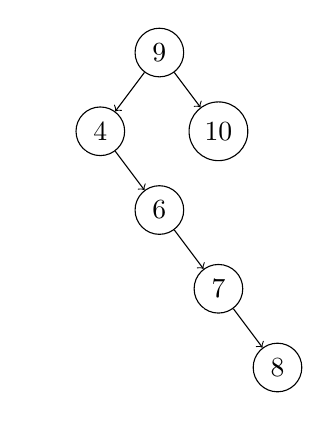
\begin{tikzpicture}[every node/.style={draw=black,circle},->,level distance=10mm]
\node{9}
	child {node {4}
		child[draw=white] {node[draw=white] {}}
		child {node {6}
			child[draw=white] {node[draw=white] {}}
			child {node {7}
				child[draw=white] {node[draw=white] {}}
				child {node {8}}
			}
		}
	}
	child {node {10}}
;
\end{tikzpicture}
}
\end{center}
Fjerningen går bra, fordi 1 og 3 kun har ett høyre barn hver. Da kan 3 sitt høyre barn bare flyttes opp til plassen 1 hadde, så er 1 og 3 fjernet.

\newpage

\subsection{SCC (oppgave 1b, H2012)}
\paragraph{1b) Anta den rettete grafen $G$ med noder $a, \dots, f$ i figuren under.}

\begin{center}
\scalebox{0.8}{
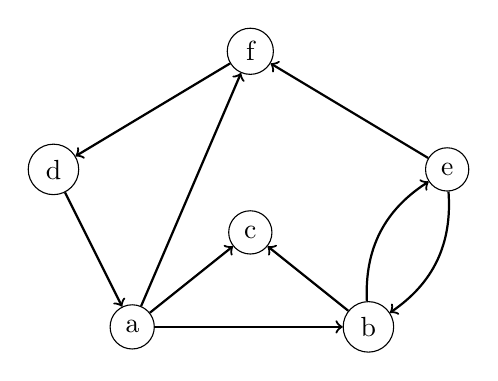
\begin{tikzpicture}[every node/.style={draw=black, circle}]
\node (a) at (0,0) {a};
\node (b) at (3,0) {b};
\node (c) at (1.5,1.2) {c};
\node (d) at (-1,2) {d};
\node (e) at (4,2) {e};
\node (f) at (1.5,3.5) {f};

\draw[->,thick] (a) to (b);
\draw[->,thick] (b) to [bend left] (e);
\draw[->,thick] (e) to [bend left] (b);
\draw[->,thick] (b) to (c);
\draw[->,thick] (a) to (c);
\draw[->,thick] (a) to (f);
\draw[->,thick] (d) to (a);
\draw[->,thick] (f) to (d);
\draw[->,thick] (e) to (f);
\end{tikzpicture}
}
\end{center}

\paragraph{1. Hvilke sterkt sammenhengende komponenter har vi i $G$? Bare lag en liste.} \{\{c\},\{d,f,e,b,a\}\}.

\paragraph{2. Vis hvordan SCCs er bestemt algoritmisk. Gi trinnene i algoritmen. Ett trinn skal tilsvare å følge en kant i grafen mellom traversering, ikke mer detaljert enn det.}

Først gjør en DFS på grafen. Starter i $a$: $a\rightarrow b \rightarrow e \rightarrow f \rightarrow d \rightarrow a \rightarrow c$. Så reversér kantene og gjør en ny DFS i avtagende rekkefølge.

\begin{minipage}{0.5\textwidth}
\scalebox{0.8}{
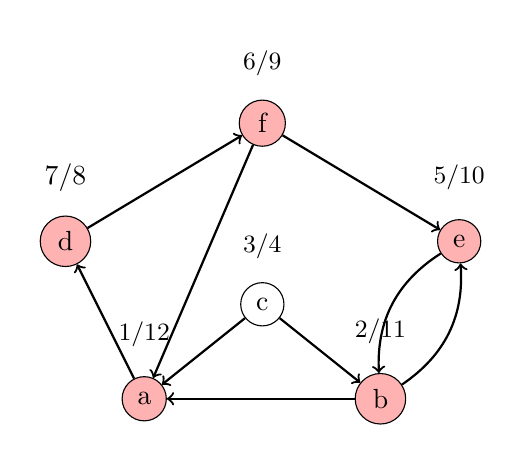
\begin{tikzpicture}[every node/.style={draw=black, circle}]
\node[fill=red!30, label={\small1/12}] (a) at (0,0) {a};
\node[fill=red!30, label={\small2/11}] (b) at (3,0) {b};
\node[label={\small3/4}] (c) at (1.5,1.2) {c};
\node[fill=red!30, label=7/8] (d) at (-1,2) {d};
\node[fill=red!30, label={\small 5/10}] (e) at (4,2) {e};
\node[fill=red!30, label={\small6/9}] (f) at (1.5,3.5) {f};

\draw[<-,thick] (a) to (b);
\draw[<-,thick] (b) to [bend left] (e);
\draw[<-,thick] (e) to [bend left] (b);
\draw[<-,thick] (b) to (c);
\draw[<-,thick] (a) to (c);
\draw[<-,thick] (a) to (f);
\draw[<-,thick] (d) to (a);
\draw[<-,thick] (f) to (d);
\draw[<-,thick] (e) to (f);
\end{tikzpicture}
}
\newline
Gjør en DFS, og så finner vi at alle, bortsett fra c henger sammen. Da er de en SCC.
\end{minipage}
\hspace{10pt}
\begin{minipage}{0.4\textwidth}
\scalebox{0.8}{
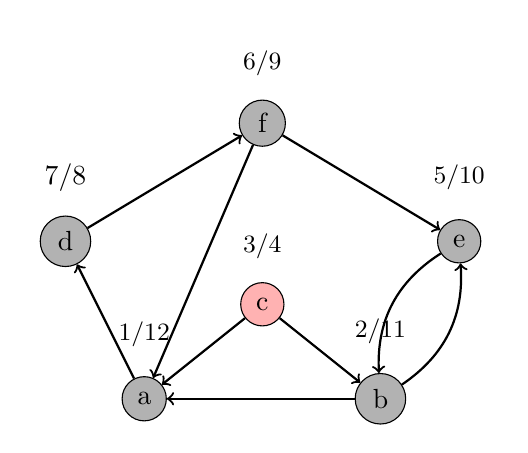
\begin{tikzpicture}[every node/.style={draw=black, circle}]
\node[fill=black!30, label={\small1/12}] (a) at (0,0) {a};
\node[fill=black!30, label={\small2/11}] (b) at (3,0) {b};
\node[fill=red!30,label={\small3/4}] (c) at (1.5,1.2) {c};
\node[fill=black!30, label=7/8] (d) at (-1,2) {d};
\node[fill=black!30, label={\small 5/10}] (e) at (4,2) {e};
\node[fill=black!30, label={\small6/9}] (f) at (1.5,3.5) {f};
g

\draw[<-,thick] (a) to (b);
\draw[<-,thick] (b) to [bend left] (e);
\draw[<-,thick] (e) to [bend left] (b);
\draw[<-,thick] (b) to (c);
\draw[<-,thick] (a) to (c);
\draw[<-,thick] (a) to (f);
\draw[<-,thick] (d) to (a);
\draw[<-,thick] (f) to (d);
\draw[<-,thick] (e) to (f);
\end{tikzpicture}
}
\newline
c er den eneste som er igjen, da er den en SCC alene.
\end{minipage}


\subsection{Grafer (oppgave 3, H2013)}
\paragraph{3a) Finn alle \textit{articulation points} for grafen under. Vis et dybde først-spenntre som starter fra node $A$ samt \textit{Num-} og \textit{Low-}numrene for hver node.}

\begin{center}
\scalebox{0.6}{
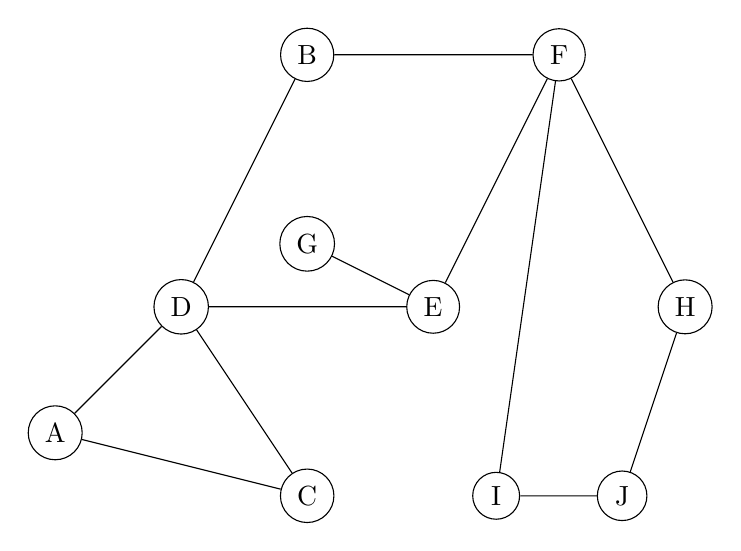
\begin{tikzpicture}[scale=1.6,every node/.style={draw=black, circle}]
\node (A) at (0,0) {A};
\node (D) at (1,1) {D};
\node (C) at (2,-0.5) {C};
\node (B) at (2,3) {B};
\node (F) at (4,3) {F};
\node (E) at (3,1) {E};
\node (G) at (2,1.5) {G};
\node (H) at (5,1) {H};
\node (J) at (4.5,-0.5) {J};
\node (I) at (3.5,-0.5) {I};

\draw (A) -- (D) -- (C) -- (A) -- (D) -- (E) -- (G) -- (E) -- (F) -- (B) -- (D) -- (E) -- (F) -- (I) -- (J) -- (H) -- (F);
\end{tikzpicture}
}
\end{center}

\begin{center}
\scalebox{0.7}{
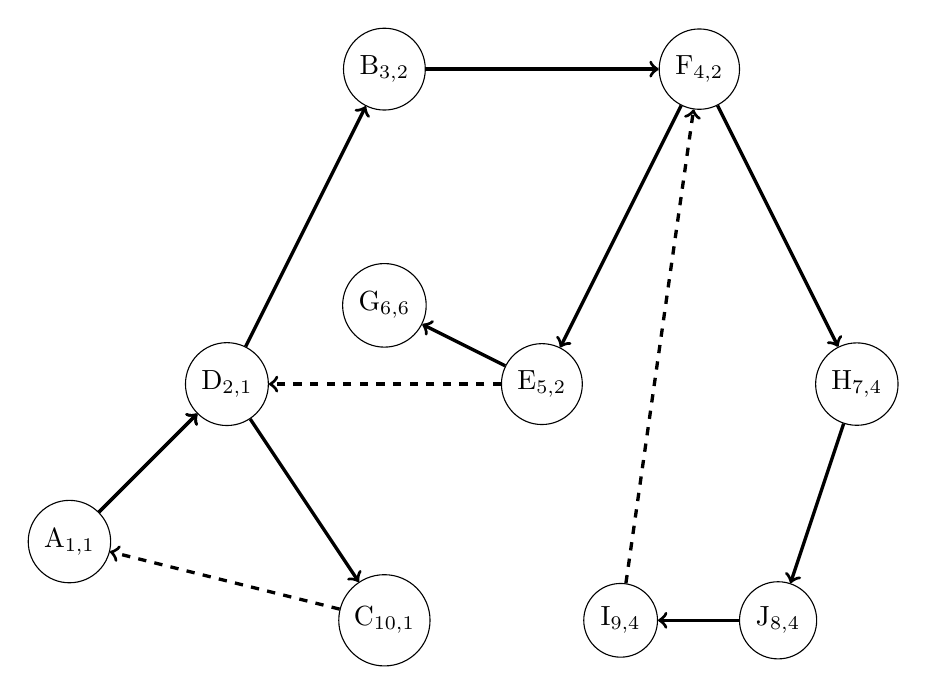
\begin{tikzpicture}[scale=2,every node/.style={draw=black, circle}]
\node (A) at (0,0) {A$_{1,1}$};
\node (D) at (1,1) {D$_{2,1}$};
\node (C) at (2,-0.5) {C$_{10,1}$};
\node (B) at (2,3) {B$_{3,2}$};
\node (F) at (4,3) {F$_{4,2}$};
\node (E) at (3,1) {E$_{5,2}$};
\node (G) at (2,1.5) {G$_{6,6}$};
\node (H) at (5,1) {H$_{7,4}$};
\node (J) at (4.5,-0.5) {J$_{8,4}$};
\node (I) at (3.5,-0.5) {I$_{9,4}$};

\draw[->, very thick] (A) to (D);
\draw[->, very thick] (A) to (D);
\draw[->, very thick] (D) to (C);
\draw[->, very thick, dashed] (C) to (A);
\draw[->, very thick] (D) to (B);
\draw[->, very thick] (B) to (F);
\draw[->, very thick] (F) to (E);
\draw[->, very thick] (E) to (G);
\draw[->, very thick] (F) to (H);
\draw[->, very thick] (J) to (I);
\draw[->, very thick] (H) to (J);
\draw[->, very thick, dashed] (I) to (F);
\draw[->, very thick, dashed] (E) to (D);
\end{tikzpicture}
}
\end{center}

E, F og D er \textit{articulation points} for denne grafen. Spenntreet over starter med A som rot-noden.

\newpage

\section{Metoder}

\begin{lstlisting}
java.util.Set<E>

boolean add(E e)				
boolean remove(Object o)		
boolean contains(Object o) 	
int size()					


java.util.List<E>

boolean add(E e)
void add(E e, int index)
boolean remove(Object o)
E remove(int index)
E get(int index)
int indexOf(Object o)
boolean contains(Object o)
int size()


java.util.Map<K,V>

boolean containsKey(Object o)
boolean containsValue(Object o)
V put(K k, V v)
V get(Object key)
V remove(Object key)
int size()
Set<K> keySet()


java.util.PriorityQueue<E>

boolean add(E e)
E peek()
E poll()
boolean contains(Object o)
int size()
\end{lstlisting}


\newpage

\begin{thebibliography}{}

\bibitem{redblack}
  Unknown,
  \emph{RedBlackBST.java}.
  algs4.cs.princeton.edu,
  \url{http://algs4.cs.princeton.edu/33balanced/RedBlackBST.java.html}

\bibitem{bm}
  Unknown,
  \emph{Boyer Moore Horspool Algorithm}.
  \url{https://www.youtube.com/watch?v=PHXAOKQk2dw}

\bibitem{sorting}
  Unknown,
  \emph{Sorting algorithm}.
  \url{http://en.wikipedia.org/wiki/Sorting_algorithm}

\bibitem{inf2220}
 Insitutt for informatikk, Universitetet i Oslo,
  \emph{INF2220--Algoritmer og datastrukturer}.
  \url{http://www.uio.no/studier/emner/matnat/ifi/INF2220/}



\end{thebibliography}

\end {document}